\documentclass[1p]{elsarticle_modified}
%\bibliographystyle{elsarticle-num}

%\usepackage[colorlinks]{hyperref}
%\usepackage{abbrmath_seonhwa} %\Abb, \Ascr, \Acal ,\Abf, \Afrak
\usepackage{amsfonts}
\usepackage{amssymb}
\usepackage{amsmath}
\usepackage{amsthm}
\usepackage{scalefnt}
\usepackage{amsbsy}
\usepackage{kotex}
\usepackage{caption}
\usepackage{subfig}
\usepackage{color}
\usepackage{graphicx}
\usepackage{xcolor} %% white, black, red, green, blue, cyan, magenta, yellow
\usepackage{float}
\usepackage{setspace}
\usepackage{hyperref}

\usepackage{tikz}
\usetikzlibrary{arrows}

\usepackage{multirow}
\usepackage{array} % fixed length table
\usepackage{hhline}

%%%%%%%%%%%%%%%%%%%%%
\makeatletter
\renewcommand*\env@matrix[1][\arraystretch]{%
	\edef\arraystretch{#1}%
	\hskip -\arraycolsep
	\let\@ifnextchar\new@ifnextchar
	\array{*\c@MaxMatrixCols c}}
\makeatother %https://tex.stackexchange.com/questions/14071/how-can-i-increase-the-line-spacing-in-a-matrix
%%%%%%%%%%%%%%%

\usepackage[normalem]{ulem}

\newcommand{\msout}[1]{\ifmmode\text{\sout{\ensuremath{#1}}}\else\sout{#1}\fi}
%SOURCE: \msout is \stkout macro in https://tex.stackexchange.com/questions/20609/strikeout-in-math-mode

\newcommand{\cancel}[1]{
	\ifmmode
	{\color{red}\msout{#1}}
	\else
	{\color{red}\sout{#1}}
	\fi
}

\newcommand{\add}[1]{
	{\color{blue}\uwave{#1}}
}

\newcommand{\replace}[2]{
	\ifmmode
	{\color{red}\msout{#1}}{\color{blue}\uwave{#2}}
	\else
	{\color{red}\sout{#1}}{\color{blue}\uwave{#2}}
	\fi
}

\newcommand{\Sol}{\mathcal{S}} %segment
\newcommand{\D}{D} %diagram
\newcommand{\A}{\mathcal{A}} %arc


%%%%%%%%%%%%%%%%%%%%%%%%%%%%%5 test

\def\sl{\operatorname{\textup{SL}}(2,\Cbb)}
\def\psl{\operatorname{\textup{PSL}}(2,\Cbb)}
\def\quan{\mkern 1mu \triangleright \mkern 1mu}

\theoremstyle{definition}
\newtheorem{thm}{Theorem}[section]
\newtheorem{prop}[thm]{Proposition}
\newtheorem{lem}[thm]{Lemma}
\newtheorem{ques}[thm]{Question}
\newtheorem{cor}[thm]{Corollary}
\newtheorem{defn}[thm]{Definition}
\newtheorem{exam}[thm]{Example}
\newtheorem{rmk}[thm]{Remark}
\newtheorem{alg}[thm]{Algorithm}

\newcommand{\I}{\sqrt{-1}}
\begin{document}

%\begin{frontmatter}
%
%\title{Boundary parabolic representations of knots up to 8 crossings}
%
%%% Group authors per affiliation:
%\author{Yunhi Cho} 
%\address{Department of Mathematics, University of Seoul, Seoul, Korea}
%\ead{yhcho@uos.ac.kr}
%
%
%\author{Seonhwa Kim} %\fnref{s_kim}}
%\address{Center for Geometry and Physics, Institute for Basic Science, Pohang, 37673, Korea}
%\ead{ryeona17@ibs.re.kr}
%
%\author{Hyuk Kim}
%\address{Department of Mathematical Sciences, Seoul National University, Seoul 08826, Korea}
%\ead{hyukkim@snu.ac.kr}
%
%\author{Seokbeom Yoon}
%\address{Department of Mathematical Sciences, Seoul National University, Seoul, 08826,  Korea}
%\ead{sbyoon15@snu.ac.kr}
%
%\begin{abstract}
%We find all boundary parabolic representation of knots up to 8 crossings.
%
%\end{abstract}
%\begin{keyword}
%    \MSC[2010] 57M25 
%\end{keyword}
%
%\end{frontmatter}

%\linenumbers
%\tableofcontents
%
\newcommand\colored[1]{\textcolor{white}{\rule[-0.35ex]{0.8em}{1.4ex}}\kern-0.8em\color{red} #1}%
%\newcommand\colored[1]{\textcolor{white}{ #1}\kern-2.17ex	\textcolor{white}{ #1}\kern-1.81ex	\textcolor{white}{ #1}\kern-2.15ex\color{red}#1	}

{\Large $\underline{12a_{0113}~(K12a_{0113})}$}

\setlength{\tabcolsep}{10pt}
\renewcommand{\arraystretch}{1.6}
\vspace{1cm}\begin{tabular}{m{100pt}>{\centering\arraybackslash}m{274pt}}
\multirow{5}{120pt}{
	\centering
	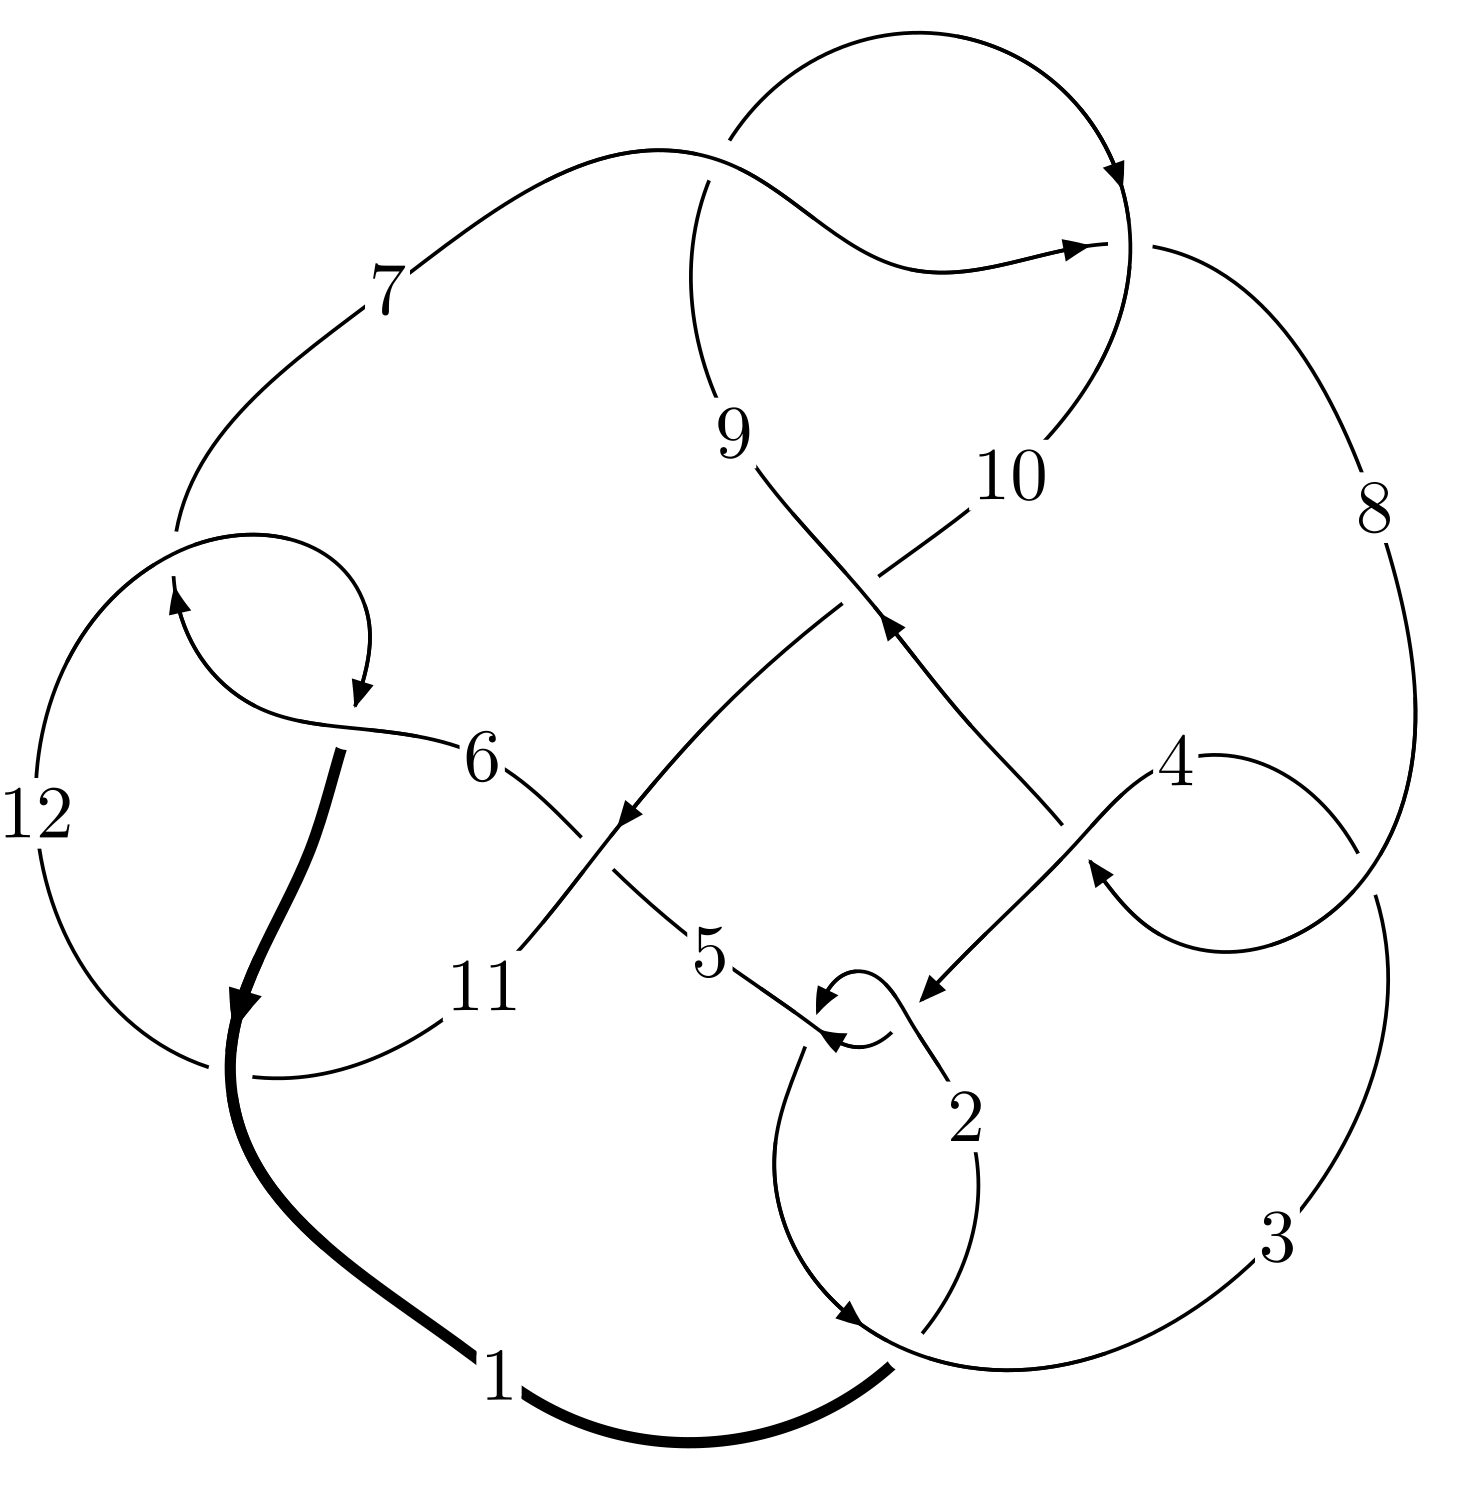
\includegraphics[width=112pt]{../../../GIT/diagram.site/Diagrams/png/914_12a_0113.png}\\
\ \ \ A knot diagram\footnotemark}&
\allowdisplaybreaks
\textbf{Linearized knot diagam} \\
\cline{2-2}
 &
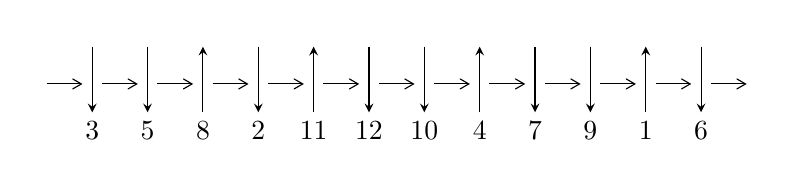
\begin{tikzpicture}[x=20pt, y=17pt]
	% nodes
	\node (C0) at (0, 0) {};
	\node (C1) at (1, 0) {};
	\node (C1U) at (1, +1) {};
	\node (C1D) at (1, -1) {3};

	\node (C2) at (2, 0) {};
	\node (C2U) at (2, +1) {};
	\node (C2D) at (2, -1) {5};

	\node (C3) at (3, 0) {};
	\node (C3U) at (3, +1) {};
	\node (C3D) at (3, -1) {8};

	\node (C4) at (4, 0) {};
	\node (C4U) at (4, +1) {};
	\node (C4D) at (4, -1) {2};

	\node (C5) at (5, 0) {};
	\node (C5U) at (5, +1) {};
	\node (C5D) at (5, -1) {11};

	\node (C6) at (6, 0) {};
	\node (C6U) at (6, +1) {};
	\node (C6D) at (6, -1) {12};

	\node (C7) at (7, 0) {};
	\node (C7U) at (7, +1) {};
	\node (C7D) at (7, -1) {10};

	\node (C8) at (8, 0) {};
	\node (C8U) at (8, +1) {};
	\node (C8D) at (8, -1) {4};

	\node (C9) at (9, 0) {};
	\node (C9U) at (9, +1) {};
	\node (C9D) at (9, -1) {7};

	\node (C10) at (10, 0) {};
	\node (C10U) at (10, +1) {};
	\node (C10D) at (10, -1) {9};

	\node (C11) at (11, 0) {};
	\node (C11U) at (11, +1) {};
	\node (C11D) at (11, -1) {1};

	\node (C12) at (12, 0) {};
	\node (C12U) at (12, +1) {};
	\node (C12D) at (12, -1) {6};
	\node (C13) at (13, 0) {};

	% arrows
	\draw[->,>={angle 60}]
	(C0) edge (C1) (C1) edge (C2) (C2) edge (C3) (C3) edge (C4) (C4) edge (C5) (C5) edge (C6) (C6) edge (C7) (C7) edge (C8) (C8) edge (C9) (C9) edge (C10) (C10) edge (C11) (C11) edge (C12) (C12) edge (C13) ;	\draw[->,>=stealth]
	(C1U) edge (C1D) (C2U) edge (C2D) (C3D) edge (C3U) (C4U) edge (C4D) (C5D) edge (C5U) (C6U) edge (C6D) (C7U) edge (C7D) (C8D) edge (C8U) (C9U) edge (C9D) (C10U) edge (C10D) (C11D) edge (C11U) (C12U) edge (C12D) ;
	\end{tikzpicture} \\
\hhline{~~} \\& 
\textbf{Solving Sequence} \\ \cline{2-2} 
 &
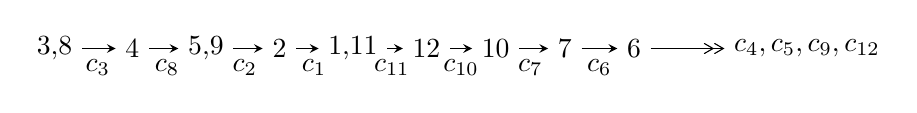
\begin{tikzpicture}[x=25pt, y=7pt]
	% node
	\node (A0) at (-1/8, 0) {3,8};
	\node (A1) at (1, 0) {4};
	\node (A2) at (33/16, 0) {5,9};
	\node (A3) at (25/8, 0) {2};
	\node (A4) at (67/16, 0) {1,11};
	\node (A5) at (21/4, 0) {12};
	\node (A6) at (25/4, 0) {10};
	\node (A7) at (29/4, 0) {7};
	\node (A8) at (33/4, 0) {6};
	\node (C1) at (1/2, -1) {$c_{3}$};
	\node (C2) at (3/2, -1) {$c_{8}$};
	\node (C3) at (21/8, -1) {$c_{2}$};
	\node (C4) at (29/8, -1) {$c_{1}$};
	\node (C5) at (19/4, -1) {$c_{11}$};
	\node (C6) at (23/4, -1) {$c_{10}$};
	\node (C7) at (27/4, -1) {$c_{7}$};
	\node (C8) at (31/4, -1) {$c_{6}$};
	\node (A9) at (43/4, 0) {$c_{4},c_{5},c_{9},c_{12}$};

	% edge
	\draw[->,>=stealth]	
	(A0) edge (A1) (A1) edge (A2) (A2) edge (A3) (A3) edge (A4) (A4) edge (A5) (A5) edge (A6) (A6) edge (A7) (A7) edge (A8) ;
	\draw[->>,>={angle 60}]	
	(A8) edge (A9);
\end{tikzpicture} \\ 

\end{tabular} \\

\footnotetext{
The image of knot diagram is generated by the software ``\textbf{Draw programme}" developed by Andrew Bartholomew(\url{http://www.layer8.co.uk/maths/draw/index.htm\#Running-draw}), where we modified some parts for our purpose(\url{https://github.com/CATsTAILs/LinksPainter}).
}\phantom \\ \newline 
\centering \textbf{Ideals for irreducible components\footnotemark of $X_{\text{par}}$} 
 
\begin{align*}
I^u_{1}&=\langle 
2.57614\times10^{61} u^{45}-5.16765\times10^{61} u^{44}+\cdots+1.04756\times10^{63} d-8.34150\times10^{62},\\
\phantom{I^u_{1}}&\phantom{= \langle  }-1.37440\times10^{61} u^{45}+5.43427\times10^{61} u^{44}+\cdots+2.09512\times10^{63} c+1.27330\times10^{63},\\
\phantom{I^u_{1}}&\phantom{= \langle  }-2.25361\times10^{61} u^{45}+4.71945\times10^{61} u^{44}+\cdots+1.04756\times10^{63} b+2.14640\times10^{62},\\
\phantom{I^u_{1}}&\phantom{= \langle  }1.04662\times10^{62} u^{45}-2.24346\times10^{62} u^{44}+\cdots+2.09512\times10^{63} a-4.78844\times10^{63},\;u^{46}-3 u^{45}+\cdots-32 u+32\rangle \\
I^u_{2}&=\langle 
-2.67306\times10^{20} a u^{37}+1.38721\times10^{19} u^{37}+\cdots+1.33819\times10^{21} a-9.87299\times10^{20},\\
\phantom{I^u_{2}}&\phantom{= \langle  }3.11246\times10^{20} a u^{37}-2.82340\times10^{20} u^{37}+\cdots+4.88853\times10^{19} a+1.51002\times10^{20},\\
\phantom{I^u_{2}}&\phantom{= \langle  }-6.51406\times10^{19} a u^{37}+1.38360\times10^{20} u^{37}+\cdots+2.42874\times10^{20} a-6.50377\times10^{20},\\
\phantom{I^u_{2}}&\phantom{= \langle  }-8.51184\times10^{19} a u^{37}+2.87125\times10^{20} u^{37}+\cdots-2.71211\times10^{21} a+1.26240\times10^{21},\;u^{38}+u^{37}+\cdots+4 u-4\rangle \\
\\
I^v_{1}&=\langle 
a,\;d,\;c- v,\;b-1,\;v^2- v+1\rangle \\
I^v_{2}&=\langle 
c,\;d+v-1,\;b,\;a-1,\;v^2- v+1\rangle \\
I^v_{3}&=\langle 
a,\;d+1,\;c+a,\;b-1,\;v+1\rangle \\
I^v_{4}&=\langle 
a,\;a^2 d+c^2 v-2 c a+c v- a+v,\;d v-1,\;c^2 v^2-2 c a v+v^2 c+a^2- a v+v^2,\;b-1\rangle \\
\end{align*}
\raggedright * 5 irreducible components of $\dim_{\mathbb{C}}=0$, with total 127 representations.\\
\raggedright * 1 irreducible components of $\dim_{\mathbb{C}}=1$ \\
\footnotetext{All coefficients of polynomials are rational numbers. But the coefficients are sometimes approximated in decimal forms when there is not enough margin.}
\newpage
\renewcommand{\arraystretch}{1}
\centering \section*{I. $I^u_{1}= \langle 2.58\times10^{61} u^{45}-5.17\times10^{61} u^{44}+\cdots+1.05\times10^{63} d-8.34\times10^{62},\;-1.37\times10^{61} u^{45}+5.43\times10^{61} u^{44}+\cdots+2.10\times10^{63} c+1.27\times10^{63},\;-2.25\times10^{61} u^{45}+4.72\times10^{61} u^{44}+\cdots+1.05\times10^{63} b+2.15\times10^{62},\;1.05\times10^{62} u^{45}-2.24\times10^{62} u^{44}+\cdots+2.10\times10^{63} a-4.79\times10^{63},\;u^{46}-3 u^{45}+\cdots-32 u+32 \rangle$}
\flushleft \textbf{(i) Arc colorings}\\
\begin{tabular}{m{7pt} m{180pt} m{7pt} m{180pt} }
\flushright $a_{3}=$&$\begin{pmatrix}1\\0\end{pmatrix}$ \\
\flushright $a_{8}=$&$\begin{pmatrix}0\\u\end{pmatrix}$ \\
\flushright $a_{4}=$&$\begin{pmatrix}1\\- u^2\end{pmatrix}$ \\
\flushright $a_{5}=$&$\begin{pmatrix}-0.0499550 u^{45}+0.107080 u^{44}+\cdots+0.105000 u+2.28551\\0.0215129 u^{45}-0.0450517 u^{44}+\cdots+0.210607 u-0.204895\end{pmatrix}$ \\
\flushright $a_{9}=$&$\begin{pmatrix}u\\- u^3+u\end{pmatrix}$ \\
\flushright $a_{2}=$&$\begin{pmatrix}-0.0499550 u^{45}+0.107080 u^{44}+\cdots+0.105000 u+2.28551\\0.0188136 u^{45}-0.0434778 u^{44}+\cdots-0.440044 u-1.16423\end{pmatrix}$ \\
\flushright $a_{1}=$&$\begin{pmatrix}-0.0311414 u^{45}+0.0636021 u^{44}+\cdots-0.335044 u+1.12129\\0.0188136 u^{45}-0.0434778 u^{44}+\cdots-0.440044 u-1.16423\end{pmatrix}$ \\
\flushright $a_{11}=$&$\begin{pmatrix}0.00655998 u^{45}-0.0259377 u^{44}+\cdots+2.00677 u-0.607746\\-0.0245918 u^{45}+0.0493302 u^{44}+\cdots+0.534931 u+0.796277\end{pmatrix}$ \\
\flushright $a_{12}=$&$\begin{pmatrix}-0.00367220 u^{45}-0.0105532 u^{44}+\cdots+1.80694 u+0.0421140\\-0.0300186 u^{45}+0.0694063 u^{44}+\cdots-0.0507359 u+1.20714\end{pmatrix}$ \\
\flushright $a_{10}=$&$\begin{pmatrix}-0.00640297 u^{45}-0.00230401 u^{44}+\cdots+2.56896 u-0.00571168\\-0.0232980 u^{45}+0.0442495 u^{44}+\cdots+1.17047 u+0.910145\end{pmatrix}$ \\
\flushright $a_{7}=$&$\begin{pmatrix}-0.0363821 u^{45}+0.0903327 u^{44}+\cdots-1.88200 u+1.60427\\-0.0298221 u^{45}+0.0643950 u^{44}+\cdots+0.124764 u+0.996524\end{pmatrix}$ \\
\flushright $a_{6}=$&$\begin{pmatrix}-0.0377231 u^{45}+0.0831509 u^{44}+\cdots-1.46595 u+1.15640\\0.0215698 u^{45}-0.0484849 u^{44}+\cdots+0.0753964 u-0.117510\end{pmatrix}$\\&\end{tabular}
\flushleft \textbf{(ii) Obstruction class $= -1$}\\~\\
\flushleft \textbf{(iii) Cusp Shapes $= -0.247381 u^{45}+0.445802 u^{44}+\cdots+4.44172 u+0.790830$}\\~\\
\newpage\renewcommand{\arraystretch}{1}
\flushleft \textbf{(iv) u-Polynomials at the component}\newline \\
\begin{tabular}{m{50pt}|m{274pt}}
Crossings & \hspace{64pt}u-Polynomials at each crossing \\
\hline $$\begin{aligned}c_{1},c_{10}\end{aligned}$$&$\begin{aligned}
&u^{46}+21 u^{45}+\cdots-4 u+1
\end{aligned}$\\
\hline $$\begin{aligned}c_{2},c_{4},c_{7}\\c_{9}\end{aligned}$$&$\begin{aligned}
&u^{46}-5 u^{45}+\cdots-2 u+1
\end{aligned}$\\
\hline $$\begin{aligned}c_{3},c_{8}\end{aligned}$$&$\begin{aligned}
&u^{46}+3 u^{45}+\cdots+32 u+32
\end{aligned}$\\
\hline $$\begin{aligned}c_{5}\end{aligned}$$&$\begin{aligned}
&u^{46}+u^{45}+\cdots+2596 u+1252
\end{aligned}$\\
\hline $$\begin{aligned}c_{6},c_{12}\end{aligned}$$&$\begin{aligned}
&u^{46}- u^{45}+\cdots+4 u+4
\end{aligned}$\\
\hline $$\begin{aligned}c_{11}\end{aligned}$$&$\begin{aligned}
&u^{46}-21 u^{45}+\cdots+40 u+16
\end{aligned}$\\
\hline
\end{tabular}\\~\\
\newpage\renewcommand{\arraystretch}{1}
\flushleft \textbf{(v) Riley Polynomials at the component}\newline \\
\begin{tabular}{m{50pt}|m{274pt}}
Crossings & \hspace{64pt}Riley Polynomials at each crossing \\
\hline $$\begin{aligned}c_{1},c_{10}\end{aligned}$$&$\begin{aligned}
&y^{46}+19 y^{45}+\cdots-72 y+1
\end{aligned}$\\
\hline $$\begin{aligned}c_{2},c_{4},c_{7}\\c_{9}\end{aligned}$$&$\begin{aligned}
&y^{46}-21 y^{45}+\cdots+4 y+1
\end{aligned}$\\
\hline $$\begin{aligned}c_{3},c_{8}\end{aligned}$$&$\begin{aligned}
&y^{46}-15 y^{45}+\cdots+4096 y+1024
\end{aligned}$\\
\hline $$\begin{aligned}c_{5}\end{aligned}$$&$\begin{aligned}
&y^{46}-3 y^{45}+\cdots-20408552 y+1567504
\end{aligned}$\\
\hline $$\begin{aligned}c_{6},c_{12}\end{aligned}$$&$\begin{aligned}
&y^{46}+21 y^{45}+\cdots-40 y+16
\end{aligned}$\\
\hline $$\begin{aligned}c_{11}\end{aligned}$$&$\begin{aligned}
&y^{46}+9 y^{45}+\cdots-5664 y+256
\end{aligned}$\\
\hline
\end{tabular}\\~\\
\newpage\flushleft \textbf{(vi) Complex Volumes and Cusp Shapes}
$$\begin{array}{c|c|c}  
\text{Solutions to }I^u_{1}& \I (\text{vol} + \sqrt{-1}CS) & \text{Cusp shape}\\
 \hline 
\begin{aligned}
u &= \phantom{-}0.248116 + 0.949341 I \\
a &= \phantom{-}0.589922 + 0.247257 I \\
b &= \phantom{-}0.441845 - 0.604328 I \\
c &= \phantom{-}0.017203 + 0.885277 I \\
d &= -0.12168 + 1.65051 I\end{aligned}
 & \phantom{-}1.66114 - 2.12776 I & \phantom{-}0.422256 + 0.234121 I \\ \hline\begin{aligned}
u &= \phantom{-}0.248116 - 0.949341 I \\
a &= \phantom{-}0.589922 - 0.247257 I \\
b &= \phantom{-}0.441845 + 0.604328 I \\
c &= \phantom{-}0.017203 - 0.885277 I \\
d &= -0.12168 - 1.65051 I\end{aligned}
 & \phantom{-}1.66114 + 2.12776 I & \phantom{-}0.422256 - 0.234121 I \\ \hline\begin{aligned}
u &= -0.642875 + 0.814816 I \\
a &= \phantom{-}0.455077 + 0.085949 I \\
b &= \phantom{-}1.121750 - 0.400729 I \\
c &= \phantom{-}0.945725 - 0.863065 I \\
d &= \phantom{-}0.751792 - 0.382393 I\end{aligned}
 & -5.93091 + 3.99675 I & -10.51051 - 4.44974 I \\ \hline\begin{aligned}
u &= -0.642875 - 0.814816 I \\
a &= \phantom{-}0.455077 - 0.085949 I \\
b &= \phantom{-}1.121750 + 0.400729 I \\
c &= \phantom{-}0.945725 + 0.863065 I \\
d &= \phantom{-}0.751792 + 0.382393 I\end{aligned}
 & -5.93091 - 3.99675 I & -10.51051 + 4.44974 I \\ \hline\begin{aligned}
u &= -0.046642 + 1.050320 I \\
a &= \phantom{-}0.521824 + 0.180773 I \\
b &= \phantom{-}0.711017 - 0.592739 I \\
c &= -0.284880 + 0.449331 I \\
d &= -1.45000 + 0.80516 I\end{aligned}
 & \phantom{-}2.04690 + 4.94372 I & -0.16550 - 7.58166 I \\ \hline\begin{aligned}
u &= -0.046642 - 1.050320 I \\
a &= \phantom{-}0.521824 - 0.180773 I \\
b &= \phantom{-}0.711017 + 0.592739 I \\
c &= -0.284880 - 0.449331 I \\
d &= -1.45000 - 0.80516 I\end{aligned}
 & \phantom{-}2.04690 - 4.94372 I & -0.16550 + 7.58166 I\\
 \hline 
 \end{array}$$\newpage$$\begin{array}{c|c|c}  
\text{Solutions to }I^u_{1}& \I (\text{vol} + \sqrt{-1}CS) & \text{Cusp shape}\\
 \hline 
\begin{aligned}
u &= \phantom{-}0.614432 + 0.696436 I \\
a &= \phantom{-}0.462583 - 0.072566 I \\
b &= \phantom{-}1.109850 + 0.330974 I \\
c &= -1.235720 - 0.572618 I \\
d &= -0.466020 + 0.040614 I\end{aligned}
 & -4.70063 + 1.01560 I & -8.78023 - 1.30126 I \\ \hline\begin{aligned}
u &= \phantom{-}0.614432 - 0.696436 I \\
a &= \phantom{-}0.462583 + 0.072566 I \\
b &= \phantom{-}1.109850 - 0.330974 I \\
c &= -1.235720 + 0.572618 I \\
d &= -0.466020 - 0.040614 I\end{aligned}
 & -4.70063 - 1.01560 I & -8.78023 + 1.30126 I \\ \hline\begin{aligned}
u &= \phantom{-}0.904459 + 0.035006 I \\
a &= \phantom{-}0.99383 - 1.43056 I \\
b &= -0.672458 + 0.471479 I \\
c &= \phantom{-}0.492096 + 0.016232 I \\
d &= \phantom{-}0.317889 - 0.738045 I\end{aligned}
 & -0.23417 + 4.06154 I & -0.42563 - 7.90074 I \\ \hline\begin{aligned}
u &= \phantom{-}0.904459 - 0.035006 I \\
a &= \phantom{-}0.99383 + 1.43056 I \\
b &= -0.672458 - 0.471479 I \\
c &= \phantom{-}0.492096 - 0.016232 I \\
d &= \phantom{-}0.317889 + 0.738045 I\end{aligned}
 & -0.23417 - 4.06154 I & -0.42563 + 7.90074 I \\ \hline\begin{aligned}
u &= \phantom{-}0.517103 + 1.038360 I \\
a &= \phantom{-}0.457040 - 0.120254 I \\
b &= \phantom{-}1.046330 + 0.538419 I \\
c &= -0.063868 - 0.817891 I \\
d &= \phantom{-}0.18483 - 1.60057 I\end{aligned}
 & -0.12548 - 4.11136 I & -2.46017 + 3.87123 I \\ \hline\begin{aligned}
u &= \phantom{-}0.517103 - 1.038360 I \\
a &= \phantom{-}0.457040 + 0.120254 I \\
b &= \phantom{-}1.046330 - 0.538419 I \\
c &= -0.063868 + 0.817891 I \\
d &= \phantom{-}0.18483 + 1.60057 I\end{aligned}
 & -0.12548 + 4.11136 I & -2.46017 - 3.87123 I\\
 \hline 
 \end{array}$$\newpage$$\begin{array}{c|c|c}  
\text{Solutions to }I^u_{1}& \I (\text{vol} + \sqrt{-1}CS) & \text{Cusp shape}\\
 \hline 
\begin{aligned}
u &= \phantom{-}0.017678 + 0.820472 I \\
a &= \phantom{-}0.576889 - 0.137924 I \\
b &= \phantom{-}0.639709 + 0.392026 I \\
c &= -0.087372 + 0.550499 I \\
d &= \phantom{-}0.487544 + 0.625296 I\end{aligned}
 & -0.79101 - 1.46703 I & -5.32252 + 4.75359 I \\ \hline\begin{aligned}
u &= \phantom{-}0.017678 - 0.820472 I \\
a &= \phantom{-}0.576889 + 0.137924 I \\
b &= \phantom{-}0.639709 - 0.392026 I \\
c &= -0.087372 - 0.550499 I \\
d &= \phantom{-}0.487544 - 0.625296 I\end{aligned}
 & -0.79101 + 1.46703 I & -5.32252 - 4.75359 I \\ \hline\begin{aligned}
u &= \phantom{-}1.006520 + 0.624064 I \\
a &= -0.40042 - 1.85496 I \\
b &= -1.111190 + 0.515094 I \\
c &= -1.121880 - 0.316865 I \\
d &= -0.633971 + 0.037265 I\end{aligned}
 & -3.52144 + 4.08819 I & -5.82465 - 4.54278 I \\ \hline\begin{aligned}
u &= \phantom{-}1.006520 - 0.624064 I \\
a &= -0.40042 + 1.85496 I \\
b &= -1.111190 - 0.515094 I \\
c &= -1.121880 + 0.316865 I \\
d &= -0.633971 - 0.037265 I\end{aligned}
 & -3.52144 - 4.08819 I & -5.82465 + 4.54278 I \\ \hline\begin{aligned}
u &= -1.071740 + 0.508840 I \\
a &= \phantom{-}0.613457 - 0.718385 I \\
b &= -0.312581 + 0.804998 I \\
c &= -1.374890 + 0.240606 I \\
d &= -0.176960 - 0.890915 I\end{aligned}
 & \phantom{-}1.98761 - 2.55534 I & -0.98949 + 1.01939 I \\ \hline\begin{aligned}
u &= -1.071740 - 0.508840 I \\
a &= \phantom{-}0.613457 + 0.718385 I \\
b &= -0.312581 - 0.804998 I \\
c &= -1.374890 - 0.240606 I \\
d &= -0.176960 + 0.890915 I\end{aligned}
 & \phantom{-}1.98761 + 2.55534 I & -0.98949 - 1.01939 I\\
 \hline 
 \end{array}$$\newpage$$\begin{array}{c|c|c}  
\text{Solutions to }I^u_{1}& \I (\text{vol} + \sqrt{-1}CS) & \text{Cusp shape}\\
 \hline 
\begin{aligned}
u &= -0.807683 + 0.082878 I \\
a &= \phantom{-}1.21197 - 1.05036 I \\
b &= -0.528808 + 0.408361 I \\
c &= -0.643863 + 0.075660 I \\
d &= -0.430989 + 0.455586 I\end{aligned}
 & -0.274017 - 1.087600 I & \phantom{-}0.651009 - 0.594713 I \\ \hline\begin{aligned}
u &= -0.807683 - 0.082878 I \\
a &= \phantom{-}1.21197 + 1.05036 I \\
b &= -0.528808 - 0.408361 I \\
c &= -0.643863 - 0.075660 I \\
d &= -0.430989 - 0.455586 I\end{aligned}
 & -0.274017 + 1.087600 I & \phantom{-}0.651009 + 0.594713 I \\ \hline\begin{aligned}
u &= -0.668777 + 1.013930 I \\
a &= \phantom{-}0.441760 + 0.107066 I \\
b &= \phantom{-}1.138080 - 0.518189 I \\
c &= \phantom{-}0.362758 - 1.282570 I \\
d &= \phantom{-}1.03682 - 1.70646 I\end{aligned}
 & -4.90536 + 6.51831 I & -8.90536 - 4.64881 I \\ \hline\begin{aligned}
u &= -0.668777 - 1.013930 I \\
a &= \phantom{-}0.441760 - 0.107066 I \\
b &= \phantom{-}1.138080 + 0.518189 I \\
c &= \phantom{-}0.362758 + 1.282570 I \\
d &= \phantom{-}1.03682 + 1.70646 I\end{aligned}
 & -4.90536 - 6.51831 I & -8.90536 + 4.64881 I \\ \hline\begin{aligned}
u &= -1.035500 + 0.682470 I \\
a &= -0.48479 + 1.75097 I \\
b &= -1.146870 - 0.530449 I \\
c &= \phantom{-}1.364230 - 0.311759 I \\
d &= \phantom{-}0.821257 + 0.527558 I\end{aligned}
 & -4.70874 - 9.62616 I & -7.79470 + 8.99124 I \\ \hline\begin{aligned}
u &= -1.035500 - 0.682470 I \\
a &= -0.48479 - 1.75097 I \\
b &= -1.146870 + 0.530449 I \\
c &= \phantom{-}1.364230 + 0.311759 I \\
d &= \phantom{-}0.821257 - 0.527558 I\end{aligned}
 & -4.70874 + 9.62616 I & -7.79470 - 8.99124 I\\
 \hline 
 \end{array}$$\newpage$$\begin{array}{c|c|c}  
\text{Solutions to }I^u_{1}& \I (\text{vol} + \sqrt{-1}CS) & \text{Cusp shape}\\
 \hline 
\begin{aligned}
u &= \phantom{-}1.224990 + 0.226721 I \\
a &= \phantom{-}0.26109 - 1.40376 I \\
b &= -0.871935 + 0.688553 I \\
c &= -0.035155 + 0.735172 I \\
d &= \phantom{-}0.474612 - 1.300260 I\end{aligned}
 & \phantom{-}3.57586 + 5.30392 I & -1.93777 - 5.96454 I \\ \hline\begin{aligned}
u &= \phantom{-}1.224990 - 0.226721 I \\
a &= \phantom{-}0.26109 + 1.40376 I \\
b &= -0.871935 - 0.688553 I \\
c &= -0.035155 - 0.735172 I \\
d &= \phantom{-}0.474612 + 1.300260 I\end{aligned}
 & \phantom{-}3.57586 - 5.30392 I & -1.93777 + 5.96454 I \\ \hline\begin{aligned}
u &= \phantom{-}1.195740 + 0.364671 I \\
a &= \phantom{-}0.555749 + 0.845299 I \\
b &= -0.456951 - 0.825982 I \\
c &= \phantom{-}1.383760 - 0.204608 I \\
d &= -0.775236 - 0.457994 I\end{aligned}
 & \phantom{-}6.39735 - 0.44189 I & \phantom{-}4.43091 + 2.06201 I \\ \hline\begin{aligned}
u &= \phantom{-}1.195740 - 0.364671 I \\
a &= \phantom{-}0.555749 - 0.845299 I \\
b &= -0.456951 + 0.825982 I \\
c &= \phantom{-}1.383760 + 0.204608 I \\
d &= -0.775236 + 0.457994 I\end{aligned}
 & \phantom{-}6.39735 + 0.44189 I & \phantom{-}4.43091 - 2.06201 I \\ \hline\begin{aligned}
u &= \phantom{-}0.687704 + 1.079720 I \\
a &= \phantom{-}0.435637 - 0.112607 I \\
b &= \phantom{-}1.151720 + 0.556193 I \\
c &= -0.16597 - 1.45383 I \\
d &= -1.16901 - 2.34716 I\end{aligned}
 & -2.74057 - 11.63170 I & -5.60201 + 8.64749 I \\ \hline\begin{aligned}
u &= \phantom{-}0.687704 - 1.079720 I \\
a &= \phantom{-}0.435637 + 0.112607 I \\
b &= \phantom{-}1.151720 - 0.556193 I \\
c &= -0.16597 + 1.45383 I \\
d &= -1.16901 + 2.34716 I\end{aligned}
 & -2.74057 + 11.63170 I & -5.60201 - 8.64749 I\\
 \hline 
 \end{array}$$\newpage$$\begin{array}{c|c|c}  
\text{Solutions to }I^u_{1}& \I (\text{vol} + \sqrt{-1}CS) & \text{Cusp shape}\\
 \hline 
\begin{aligned}
u &= \phantom{-}1.158970 + 0.578549 I \\
a &= \phantom{-}0.544904 + 0.699989 I \\
b &= -0.307535 - 0.889547 I \\
c &= \phantom{-}1.64315 + 0.27736 I \\
d &= \phantom{-}0.06540 - 1.58776 I\end{aligned}
 & \phantom{-}4.42926 + 7.47789 I & \phantom{-}1.74286 - 4.84208 I \\ \hline\begin{aligned}
u &= \phantom{-}1.158970 - 0.578549 I \\
a &= \phantom{-}0.544904 - 0.699989 I \\
b &= -0.307535 + 0.889547 I \\
c &= \phantom{-}1.64315 - 0.27736 I \\
d &= \phantom{-}0.06540 + 1.58776 I\end{aligned}
 & \phantom{-}4.42926 - 7.47789 I & \phantom{-}1.74286 + 4.84208 I \\ \hline\begin{aligned}
u &= -1.311140 + 0.102134 I \\
a &= \phantom{-}0.311679 + 1.221780 I \\
b &= -0.803961 - 0.768470 I \\
c &= -0.364729 + 0.984342 I \\
d &= \phantom{-}0.02550 - 1.73526 I\end{aligned}
 & \phantom{-}7.51022 - 1.50301 I & \phantom{-}3.10935 + 2.27720 I \\ \hline\begin{aligned}
u &= -1.311140 - 0.102134 I \\
a &= \phantom{-}0.311679 - 1.221780 I \\
b &= -0.803961 + 0.768470 I \\
c &= -0.364729 - 0.984342 I \\
d &= \phantom{-}0.02550 + 1.73526 I\end{aligned}
 & \phantom{-}7.51022 + 1.50301 I & \phantom{-}3.10935 - 2.27720 I \\ \hline\begin{aligned}
u &= -0.435796 + 0.485308 I \\
a &= \phantom{-}0.857168 - 0.309306 I \\
b &= \phantom{-}0.032227 + 0.372475 I \\
c &= -0.440235 + 0.495589 I \\
d &= -0.501506 + 0.464460 I\end{aligned}
 & \phantom{-}0.084212 - 1.381070 I & \phantom{-}0.30299 + 4.86269 I \\ \hline\begin{aligned}
u &= -0.435796 - 0.485308 I \\
a &= \phantom{-}0.857168 + 0.309306 I \\
b &= \phantom{-}0.032227 - 0.372475 I \\
c &= -0.440235 - 0.495589 I \\
d &= -0.501506 - 0.464460 I\end{aligned}
 & \phantom{-}0.084212 + 1.381070 I & \phantom{-}0.30299 - 4.86269 I\\
 \hline 
 \end{array}$$\newpage$$\begin{array}{c|c|c}  
\text{Solutions to }I^u_{1}& \I (\text{vol} + \sqrt{-1}CS) & \text{Cusp shape}\\
 \hline 
\begin{aligned}
u &= -1.316840 + 0.304432 I \\
a &= \phantom{-}0.116039 + 1.346760 I \\
b &= -0.936495 - 0.737050 I \\
c &= \phantom{-}0.307546 + 1.028890 I \\
d &= -1.03275 - 1.46411 I\end{aligned}
 & \phantom{-}6.69471 - 9.89538 I & \phantom{-}1.12698 + 9.02462 I \\ \hline\begin{aligned}
u &= -1.316840 - 0.304432 I \\
a &= \phantom{-}0.116039 - 1.346760 I \\
b &= -0.936495 + 0.737050 I \\
c &= \phantom{-}0.307546 - 1.028890 I \\
d &= -1.03275 + 1.46411 I\end{aligned}
 & \phantom{-}6.69471 + 9.89538 I & \phantom{-}1.12698 - 9.02462 I \\ \hline\begin{aligned}
u &= -1.118430 + 0.781907 I \\
a &= -0.55775 + 1.54027 I \\
b &= -1.207840 - 0.573976 I \\
c &= \phantom{-}1.86293 - 0.18421 I \\
d &= \phantom{-}0.89762 + 1.88496 I\end{aligned}
 & -3.44989 - 13.07100 I & -7.52581 + 7.90184 I \\ \hline\begin{aligned}
u &= -1.118430 - 0.781907 I \\
a &= -0.55775 - 1.54027 I \\
b &= -1.207840 + 0.573976 I \\
c &= \phantom{-}1.86293 + 0.18421 I \\
d &= \phantom{-}0.89762 - 1.88496 I\end{aligned}
 & -3.44989 + 13.07100 I & -7.52581 - 7.90184 I \\ \hline\begin{aligned}
u &= \phantom{-}1.166960 + 0.709743 I \\
a &= -0.42776 - 1.53120 I \\
b &= -1.169240 + 0.605803 I \\
c &= -1.67165 + 0.11957 I \\
d &= \phantom{-}0.04746 + 1.51937 I\end{aligned}
 & \phantom{-}1.96462 + 10.42030 I & \phantom{-0.000000 } 0. - 7.01224 I \\ \hline\begin{aligned}
u &= \phantom{-}1.166960 - 0.709743 I \\
a &= -0.42776 + 1.53120 I \\
b &= -1.169240 - 0.605803 I \\
c &= -1.67165 - 0.11957 I \\
d &= \phantom{-}0.04746 - 1.51937 I\end{aligned}
 & \phantom{-}1.96462 - 10.42030 I & \phantom{-0.000000 -}0. + 7.01224 I\\
 \hline 
 \end{array}$$\newpage$$\begin{array}{c|c|c}  
\text{Solutions to }I^u_{1}& \I (\text{vol} + \sqrt{-1}CS) & \text{Cusp shape}\\
 \hline 
\begin{aligned}
u &= \phantom{-}1.144720 + 0.813548 I \\
a &= -0.57296 - 1.48160 I \\
b &= -1.227060 + 0.587138 I \\
c &= -2.03119 - 0.14199 I \\
d &= -0.89891 + 2.41812 I\end{aligned}
 & -1.2351 + 18.4885 I & -4.00000 - 11.60486 I \\ \hline\begin{aligned}
u &= \phantom{-}1.144720 - 0.813548 I \\
a &= -0.57296 + 1.48160 I \\
b &= -1.227060 - 0.587138 I \\
c &= -2.03119 + 0.14199 I \\
d &= -0.89891 - 2.41812 I\end{aligned}
 & -1.2351 - 18.4885 I & -4.00000 + 11.60486 I \\ \hline\begin{aligned}
u &= \phantom{-}0.068034 + 0.485475 I \\
a &= \phantom{-}0.537064 - 0.015658 I \\
b &= \phantom{-}0.860393 + 0.054239 I \\
c &= -0.358003 + 1.358470 I \\
d &= \phantom{-}0.046305 + 0.232893 I\end{aligned}
 & -2.91211 - 2.24138 I & -11.31463 + 3.80305 I \\ \hline\begin{aligned}
u &= \phantom{-}0.068034 - 0.485475 I \\
a &= \phantom{-}0.537064 + 0.015658 I \\
b &= \phantom{-}0.860393 - 0.054239 I \\
c &= -0.358003 - 1.358470 I \\
d &= \phantom{-}0.046305 - 0.232893 I\end{aligned}
 & -2.91211 + 2.24138 I & -11.31463 - 3.80305 I\\
 \hline 
 \end{array}$$\newpage\newpage\renewcommand{\arraystretch}{1}
\centering \section*{II. $I^u_{2}= \langle -2.67\times10^{20} a u^{37}+1.39\times10^{19} u^{37}+\cdots+1.34\times10^{21} a-9.87\times10^{20},\;3.11\times10^{20} a u^{37}-2.82\times10^{20} u^{37}+\cdots+4.89\times10^{19} a+1.51\times10^{20},\;-6.51\times10^{19} a u^{37}+1.38\times10^{20} u^{37}+\cdots+2.43\times10^{20} a-6.50\times10^{20},\;-8.51\times10^{19} a u^{37}+2.87\times10^{20} u^{37}+\cdots-2.71\times10^{21} a+1.26\times10^{21},\;u^{38}+u^{37}+\cdots+4 u-4 \rangle$}
\flushleft \textbf{(i) Arc colorings}\\
\begin{tabular}{m{7pt} m{180pt} m{7pt} m{180pt} }
\flushright $a_{3}=$&$\begin{pmatrix}1\\0\end{pmatrix}$ \\
\flushright $a_{8}=$&$\begin{pmatrix}0\\u\end{pmatrix}$ \\
\flushright $a_{4}=$&$\begin{pmatrix}1\\- u^2\end{pmatrix}$ \\
\flushright $a_{5}=$&$\begin{pmatrix}a\\0.351994 a u^{37}-0.747643 u^{37}+\cdots-1.31240 a+3.51438\end{pmatrix}$ \\
\flushright $a_{9}=$&$\begin{pmatrix}u\\- u^3+u\end{pmatrix}$ \\
\flushright $a_{2}=$&$\begin{pmatrix}a\\-0.351994 a u^{37}+0.747643 u^{37}+\cdots+1.31240 a-3.51438\end{pmatrix}$ \\
\flushright $a_{1}=$&$\begin{pmatrix}-0.351994 a u^{37}+0.747643 u^{37}+\cdots+2.31240 a-3.51438\\-0.351994 a u^{37}+0.747643 u^{37}+\cdots+1.31240 a-3.51438\end{pmatrix}$ \\
\flushright $a_{11}=$&$\begin{pmatrix}-0.840926 a u^{37}+0.762827 u^{37}+\cdots-0.132078 a-0.407976\\0.722207 a u^{37}-0.0374795 u^{37}+\cdots-3.61552 a+2.66749\end{pmatrix}$ \\
\flushright $a_{12}=$&$\begin{pmatrix}0.717046 a u^{37}-0.375927 u^{37}+\cdots-6.28667 a+4.45469\\1.61990 a u^{37}-1.17623 u^{37}+\cdots-6.25098 a+7.53015\end{pmatrix}$ \\
\flushright $a_{10}=$&$\begin{pmatrix}-0.328099 a u^{37}+0.250000 u^{37}+\cdots-1.54005 a+1\\0.512827 a u^{37}+0.171901 u^{37}+\cdots-1.40798 a+0.459946\end{pmatrix}$ \\
\flushright $a_{7}=$&$\begin{pmatrix}0.328099 a u^{37}-0.0780990 u^{37}+\cdots+1.54005 a-0.540054\\-0.512827 a u^{37}+0.684728 u^{37}+\cdots+1.40798 a-0.948030\end{pmatrix}$ \\
\flushright $a_{6}=$&$\begin{pmatrix}1.56275 a u^{37}-0.842508 u^{37}+\cdots-1.04475 a+2.32445\\-0.332058 a u^{37}-0.0145277 u^{37}+\cdots+2.86819 a+1.41585\end{pmatrix}$\\&\end{tabular}
\flushleft \textbf{(ii) Obstruction class $= -1$}\\~\\
\flushleft \textbf{(iii) Cusp Shapes $= \frac{125334397169543797937}{92530874909565185306} u^{37}+\frac{144830212205814099033}{92530874909565185306} u^{36}+\cdots+\frac{34223567447539124627}{92530874909565185306} u-\frac{228286816014379276432}{46265437454782592653}$}\\~\\
\newpage\renewcommand{\arraystretch}{1}
\flushleft \textbf{(iv) u-Polynomials at the component}\newline \\
\begin{tabular}{m{50pt}|m{274pt}}
Crossings & \hspace{64pt}u-Polynomials at each crossing \\
\hline $$\begin{aligned}c_{1}\end{aligned}$$&$\begin{aligned}
&u^{76}+43 u^{75}+\cdots+800 u+256
\end{aligned}$\\
\hline $$\begin{aligned}c_{2},c_{7}\end{aligned}$$&$\begin{aligned}
&u^{76}-3 u^{75}+\cdots+104 u-16
\end{aligned}$\\
\hline $$\begin{aligned}c_{3}\end{aligned}$$&$\begin{aligned}
&(u^{38}- u^{37}+\cdots-4 u-4)^{2}
\end{aligned}$\\
\hline $$\begin{aligned}c_{4},c_{9}\end{aligned}$$&$\begin{aligned}
&- u^{76}-3 u^{75}+\cdots+104 u+16
\end{aligned}$\\
\hline $$\begin{aligned}c_{5}\end{aligned}$$&$\begin{aligned}
&(u^{38}+2 u^{37}+\cdots+37 u+17)^{2}
\end{aligned}$\\
\hline $$\begin{aligned}c_{6}\end{aligned}$$&$\begin{aligned}
&(u^{38}-2 u^{37}+\cdots-5 u+1)^{2}
\end{aligned}$\\
\hline $$\begin{aligned}c_{8}\end{aligned}$$&$\begin{aligned}
&(u^{38}+u^{37}+\cdots+4 u-4)^{2}
\end{aligned}$\\
\hline $$\begin{aligned}c_{10}\end{aligned}$$&$\begin{aligned}
&u^{76}-43 u^{75}+\cdots-800 u+256
\end{aligned}$\\
\hline $$\begin{aligned}c_{11}\end{aligned}$$&$\begin{aligned}
&(u^{38}+18 u^{37}+\cdots-5 u+1)^{2}
\end{aligned}$\\
\hline $$\begin{aligned}c_{12}\end{aligned}$$&$\begin{aligned}
&(u^{38}+2 u^{37}+\cdots+5 u+1)^{2}
\end{aligned}$\\
\hline
\end{tabular}\\~\\
\newpage\renewcommand{\arraystretch}{1}
\flushleft \textbf{(v) Riley Polynomials at the component}\newline \\
\begin{tabular}{m{50pt}|m{274pt}}
Crossings & \hspace{64pt}Riley Polynomials at each crossing \\
\hline $$\begin{aligned}c_{1},c_{10}\end{aligned}$$&$\begin{aligned}
&y^{76}-23 y^{75}+\cdots-1516032 y+65536
\end{aligned}$\\
\hline $$\begin{aligned}c_{2},c_{4},c_{7}\\c_{9}\end{aligned}$$&$\begin{aligned}
&y^{76}-43 y^{75}+\cdots-800 y+256
\end{aligned}$\\
\hline $$\begin{aligned}c_{3},c_{8}\end{aligned}$$&$\begin{aligned}
&(y^{38}-15 y^{37}+\cdots-72 y+16)^{2}
\end{aligned}$\\
\hline $$\begin{aligned}c_{5}\end{aligned}$$&$\begin{aligned}
&(y^{38}-6 y^{37}+\cdots-6333 y+289)^{2}
\end{aligned}$\\
\hline $$\begin{aligned}c_{6},c_{12}\end{aligned}$$&$\begin{aligned}
&(y^{38}+18 y^{37}+\cdots-5 y+1)^{2}
\end{aligned}$\\
\hline $$\begin{aligned}c_{11}\end{aligned}$$&$\begin{aligned}
&(y^{38}+6 y^{37}+\cdots-61 y+1)^{2}
\end{aligned}$\\
\hline
\end{tabular}\\~\\
\newpage\flushleft \textbf{(vi) Complex Volumes and Cusp Shapes}
$$\begin{array}{c|c|c}  
\text{Solutions to }I^u_{2}& \I (\text{vol} + \sqrt{-1}CS) & \text{Cusp shape}\\
 \hline 
\begin{aligned}
u &= -0.718175 + 0.689913 I \\
a &= \phantom{-}0.450629 + 0.069011 I \\
b &= \phantom{-}1.168270 - 0.332058 I \\
c &= \phantom{-}0.82426 - 1.31061 I \\
d &= \phantom{-}1.77249 - 1.85878 I\end{aligned}
 & -6.09366 - 1.46931 I & -10.87065 + 3.08473 I \\ \hline\begin{aligned}
u &= -0.718175 + 0.689913 I \\
a &= -1.05848 + 2.42146 I \\
b &= -1.151560 - 0.346723 I \\
c &= \phantom{-}1.44273 - 0.85052 I \\
d &= \phantom{-}0.779906 + 0.302096 I\end{aligned}
 & -6.09366 - 1.46931 I & -10.87065 + 3.08473 I \\ \hline\begin{aligned}
u &= -0.718175 - 0.689913 I \\
a &= \phantom{-}0.450629 - 0.069011 I \\
b &= \phantom{-}1.168270 + 0.332058 I \\
c &= \phantom{-}0.82426 + 1.31061 I \\
d &= \phantom{-}1.77249 + 1.85878 I\end{aligned}
 & -6.09366 + 1.46931 I & -10.87065 - 3.08473 I \\ \hline\begin{aligned}
u &= -0.718175 - 0.689913 I \\
a &= -1.05848 - 2.42146 I \\
b &= -1.151560 + 0.346723 I \\
c &= \phantom{-}1.44273 + 0.85052 I \\
d &= \phantom{-}0.779906 - 0.302096 I\end{aligned}
 & -6.09366 + 1.46931 I & -10.87065 - 3.08473 I \\ \hline\begin{aligned}
u &= -0.257524 + 0.984493 I \\
a &= \phantom{-}0.578727 - 0.253722 I \\
b &= \phantom{-}0.449354 + 0.635417 I \\
c &= -0.0473997 - 0.0121555 I \\
d &= -1.051440 - 0.287772 I\end{aligned}
 & \phantom{-}1.60581 - 0.49664 I & \phantom{-}0.272784 + 1.115032 I \\ \hline\begin{aligned}
u &= -0.257524 + 0.984493 I \\
a &= \phantom{-}0.498072 + 0.137191 I \\
b &= \phantom{-}0.866155 - 0.514022 I \\
c &= \phantom{-}0.017878 + 0.930985 I \\
d &= \phantom{-}0.15505 + 1.83052 I\end{aligned}
 & \phantom{-}1.60581 - 0.49664 I & \phantom{-}0.272784 + 1.115032 I\\
 \hline 
 \end{array}$$\newpage$$\begin{array}{c|c|c}  
\text{Solutions to }I^u_{2}& \I (\text{vol} + \sqrt{-1}CS) & \text{Cusp shape}\\
 \hline 
\begin{aligned}
u &= -0.257524 - 0.984493 I \\
a &= \phantom{-}0.578727 + 0.253722 I \\
b &= \phantom{-}0.449354 - 0.635417 I \\
c &= -0.0473997 + 0.0121555 I \\
d &= -1.051440 + 0.287772 I\end{aligned}
 & \phantom{-}1.60581 + 0.49664 I & \phantom{-}0.272784 - 1.115032 I \\ \hline\begin{aligned}
u &= -0.257524 - 0.984493 I \\
a &= \phantom{-}0.498072 - 0.137191 I \\
b &= \phantom{-}0.866155 + 0.514022 I \\
c &= \phantom{-}0.017878 - 0.930985 I \\
d &= \phantom{-}0.15505 - 1.83052 I\end{aligned}
 & \phantom{-}1.60581 + 0.49664 I & \phantom{-}0.272784 - 1.115032 I \\ \hline\begin{aligned}
u &= -0.924425 + 0.450549 I \\
a &= \phantom{-}0.733764 - 0.695514 I \\
b &= -0.282136 + 0.680443 I \\
c &= \phantom{-}2.44374 - 0.86916 I \\
d &= -0.05679 + 1.53145 I\end{aligned}
 & -0.88516 - 3.95746 I & -1.72480 + 4.57056 I \\ \hline\begin{aligned}
u &= -0.924425 + 0.450549 I \\
a &= \phantom{-}0.434246 + 0.040729 I \\
b &= \phantom{-}1.282760 - 0.214107 I \\
c &= -1.063930 + 0.292390 I \\
d &= -0.442706 - 0.285409 I\end{aligned}
 & -0.88516 - 3.95746 I & -1.72480 + 4.57056 I \\ \hline\begin{aligned}
u &= -0.924425 - 0.450549 I \\
a &= \phantom{-}0.733764 + 0.695514 I \\
b &= -0.282136 - 0.680443 I \\
c &= \phantom{-}2.44374 + 0.86916 I \\
d &= -0.05679 - 1.53145 I\end{aligned}
 & -0.88516 + 3.95746 I & -1.72480 - 4.57056 I \\ \hline\begin{aligned}
u &= -0.924425 - 0.450549 I \\
a &= \phantom{-}0.434246 - 0.040729 I \\
b &= \phantom{-}1.282760 + 0.214107 I \\
c &= -1.063930 - 0.292390 I \\
d &= -0.442706 + 0.285409 I\end{aligned}
 & -0.88516 + 3.95746 I & -1.72480 - 4.57056 I\\
 \hline 
 \end{array}$$\newpage$$\begin{array}{c|c|c}  
\text{Solutions to }I^u_{2}& \I (\text{vol} + \sqrt{-1}CS) & \text{Cusp shape}\\
 \hline 
\begin{aligned}
u &= \phantom{-}0.531079 + 0.883531 I \\
a &= \phantom{-}0.622511 + 0.357737 I \\
b &= \phantom{-}0.207598 - 0.693967 I \\
c &= -0.558583 - 0.645103 I \\
d &= -0.214583 - 0.739308 I\end{aligned}
 & -2.26472 - 1.90334 I & -6.18021 + 1.07076 I \\ \hline\begin{aligned}
u &= \phantom{-}0.531079 + 0.883531 I \\
a &= \phantom{-}0.465715 - 0.099917 I \\
b &= \phantom{-}1.052750 + 0.440407 I \\
c &= \phantom{-}0.451533 + 1.059860 I \\
d &= \phantom{-}1.21258 + 1.38512 I\end{aligned}
 & -2.26472 - 1.90334 I & -6.18021 + 1.07076 I \\ \hline\begin{aligned}
u &= \phantom{-}0.531079 - 0.883531 I \\
a &= \phantom{-}0.622511 - 0.357737 I \\
b &= \phantom{-}0.207598 + 0.693967 I \\
c &= -0.558583 + 0.645103 I \\
d &= -0.214583 + 0.739308 I\end{aligned}
 & -2.26472 + 1.90334 I & -6.18021 - 1.07076 I \\ \hline\begin{aligned}
u &= \phantom{-}0.531079 - 0.883531 I \\
a &= \phantom{-}0.465715 + 0.099917 I \\
b &= \phantom{-}1.052750 - 0.440407 I \\
c &= \phantom{-}0.451533 - 1.059860 I \\
d &= \phantom{-}1.21258 - 1.38512 I\end{aligned}
 & -2.26472 + 1.90334 I & -6.18021 - 1.07076 I \\ \hline\begin{aligned}
u &= -0.860778 + 0.429023 I \\
a &= \phantom{-}0.789089 - 0.671236 I \\
b &= -0.264746 + 0.625441 I \\
c &= \phantom{-}0.320925 - 0.473124 I \\
d &= \phantom{-}0.139948 - 1.119540 I\end{aligned}
 & -1.135440 + 0.390890 I & -2.15175 + 1.14697 I \\ \hline\begin{aligned}
u &= -0.860778 + 0.429023 I \\
a &= \phantom{-}0.07205 + 2.35819 I \\
b &= -0.987057 - 0.423659 I \\
c &= -0.954913 + 0.311920 I \\
d &= -0.508328 - 0.109971 I\end{aligned}
 & -1.135440 + 0.390890 I & -2.15175 + 1.14697 I\\
 \hline 
 \end{array}$$\newpage$$\begin{array}{c|c|c}  
\text{Solutions to }I^u_{2}& \I (\text{vol} + \sqrt{-1}CS) & \text{Cusp shape}\\
 \hline 
\begin{aligned}
u &= -0.860778 - 0.429023 I \\
a &= \phantom{-}0.789089 + 0.671236 I \\
b &= -0.264746 - 0.625441 I \\
c &= \phantom{-}0.320925 + 0.473124 I \\
d &= \phantom{-}0.139948 + 1.119540 I\end{aligned}
 & -1.135440 - 0.390890 I & -2.15175 - 1.14697 I \\ \hline\begin{aligned}
u &= -0.860778 - 0.429023 I \\
a &= \phantom{-}0.07205 - 2.35819 I \\
b &= -0.987057 + 0.423659 I \\
c &= -0.954913 - 0.311920 I \\
d &= -0.508328 + 0.109971 I\end{aligned}
 & -1.135440 - 0.390890 I & -2.15175 - 1.14697 I \\ \hline\begin{aligned}
u &= \phantom{-}0.959864 + 0.423605 I \\
a &= \phantom{-}0.431319 - 0.037774 I \\
b &= \phantom{-}1.300820 + 0.201498 I \\
c &= -0.436644 - 0.188137 I \\
d &= -0.003550 - 0.813354 I\end{aligned}
 & -0.93346 + 1.43399 I & -1.64648 - 2.88902 I \\ \hline\begin{aligned}
u &= \phantom{-}0.959864 + 0.423605 I \\
a &= \phantom{-}0.07049 - 2.03730 I \\
b &= -0.983037 + 0.490258 I \\
c &= -2.57502 - 0.87790 I \\
d &= \phantom{-}0.26331 + 1.68900 I\end{aligned}
 & -0.93346 + 1.43399 I & -1.64648 - 2.88902 I \\ \hline\begin{aligned}
u &= \phantom{-}0.959864 - 0.423605 I \\
a &= \phantom{-}0.431319 + 0.037774 I \\
b &= \phantom{-}1.300820 - 0.201498 I \\
c &= -0.436644 + 0.188137 I \\
d &= -0.003550 + 0.813354 I\end{aligned}
 & -0.93346 - 1.43399 I & -1.64648 + 2.88902 I \\ \hline\begin{aligned}
u &= \phantom{-}0.959864 - 0.423605 I \\
a &= \phantom{-}0.07049 + 2.03730 I \\
b &= -0.983037 - 0.490258 I \\
c &= -2.57502 + 0.87790 I \\
d &= \phantom{-}0.26331 - 1.68900 I\end{aligned}
 & -0.93346 - 1.43399 I & -1.64648 + 2.88902 I\\
 \hline 
 \end{array}$$\newpage$$\begin{array}{c|c|c}  
\text{Solutions to }I^u_{2}& \I (\text{vol} + \sqrt{-1}CS) & \text{Cusp shape}\\
 \hline 
\begin{aligned}
u &= \phantom{-}0.590924 + 0.743055 I \\
a &= \phantom{-}0.464137 - 0.079085 I \\
b &= \phantom{-}1.093750 + 0.356756 I \\
c &= -0.73068 - 1.75542 I \\
d &= -2.09697 - 2.99942 I\end{aligned}
 & -4.63851 - 3.34557 I & -8.53398 + 2.94107 I \\ \hline\begin{aligned}
u &= \phantom{-}0.590924 + 0.743055 I \\
a &= -1.64730 - 2.48133 I \\
b &= -1.185700 + 0.279725 I \\
c &= -1.063010 - 0.587695 I \\
d &= -0.450613 - 0.143094 I\end{aligned}
 & -4.63851 - 3.34557 I & -8.53398 + 2.94107 I \\ \hline\begin{aligned}
u &= \phantom{-}0.590924 - 0.743055 I \\
a &= \phantom{-}0.464137 + 0.079085 I \\
b &= \phantom{-}1.093750 - 0.356756 I \\
c &= -0.73068 + 1.75542 I \\
d &= -2.09697 + 2.99942 I\end{aligned}
 & -4.63851 + 3.34557 I & -8.53398 - 2.94107 I \\ \hline\begin{aligned}
u &= \phantom{-}0.590924 - 0.743055 I \\
a &= -1.64730 + 2.48133 I \\
b &= -1.185700 - 0.279725 I \\
c &= -1.063010 + 0.587695 I \\
d &= -0.450613 + 0.143094 I\end{aligned}
 & -4.63851 + 3.34557 I & -8.53398 - 2.94107 I \\ \hline\begin{aligned}
u &= -0.944268 + 0.080074 I \\
a &= \phantom{-}0.90488 - 1.15379 I \\
b &= -0.579133 + 0.536637 I \\
c &= \phantom{-}2.95149 - 0.14973 I \\
d &= -1.41848 + 0.38074 I\end{aligned}
 & \phantom{-}0.25240 + 2.75914 I & \phantom{-}1.19764 - 4.35912 I \\ \hline\begin{aligned}
u &= -0.944268 + 0.080074 I \\
a &= \phantom{-}0.434964 + 0.007055 I \\
b &= \phantom{-}1.298440 - 0.037280 I \\
c &= -0.661782 - 0.078108 I \\
d &= -0.169418 + 0.540287 I\end{aligned}
 & \phantom{-}0.25240 + 2.75914 I & \phantom{-}1.19764 - 4.35912 I\\
 \hline 
 \end{array}$$\newpage$$\begin{array}{c|c|c}  
\text{Solutions to }I^u_{2}& \I (\text{vol} + \sqrt{-1}CS) & \text{Cusp shape}\\
 \hline 
\begin{aligned}
u &= -0.944268 - 0.080074 I \\
a &= \phantom{-}0.90488 + 1.15379 I \\
b &= -0.579133 - 0.536637 I \\
c &= \phantom{-}2.95149 + 0.14973 I \\
d &= -1.41848 - 0.38074 I\end{aligned}
 & \phantom{-}0.25240 - 2.75914 I & \phantom{-}1.19764 + 4.35912 I \\ \hline\begin{aligned}
u &= -0.944268 - 0.080074 I \\
a &= \phantom{-}0.434964 - 0.007055 I \\
b &= \phantom{-}1.298440 + 0.037280 I \\
c &= -0.661782 + 0.078108 I \\
d &= -0.169418 - 0.540287 I\end{aligned}
 & \phantom{-}0.25240 - 2.75914 I & \phantom{-}1.19764 + 4.35912 I \\ \hline\begin{aligned}
u &= \phantom{-}0.932230 + 0.544110 I \\
a &= \phantom{-}0.681744 + 0.643239 I \\
b &= -0.223996 - 0.732175 I \\
c &= -0.757090 - 0.432327 I \\
d &= -0.505611 - 0.637960 I\end{aligned}
 & -2.05024 + 4.86305 I & -4.53119 - 6.13263 I \\ \hline\begin{aligned}
u &= \phantom{-}0.932230 + 0.544110 I \\
a &= -0.26957 - 2.08849 I \\
b &= -1.060790 + 0.470969 I \\
c &= \phantom{-}1.152600 + 0.439830 I \\
d &= \phantom{-}0.702756 - 0.492106 I\end{aligned}
 & -2.05024 + 4.86305 I & -4.53119 - 6.13263 I \\ \hline\begin{aligned}
u &= \phantom{-}0.932230 - 0.544110 I \\
a &= \phantom{-}0.681744 - 0.643239 I \\
b &= -0.223996 + 0.732175 I \\
c &= -0.757090 + 0.432327 I \\
d &= -0.505611 + 0.637960 I\end{aligned}
 & -2.05024 - 4.86305 I & -4.53119 + 6.13263 I \\ \hline\begin{aligned}
u &= \phantom{-}0.932230 - 0.544110 I \\
a &= -0.26957 + 2.08849 I \\
b &= -1.060790 - 0.470969 I \\
c &= \phantom{-}1.152600 - 0.439830 I \\
d &= \phantom{-}0.702756 + 0.492106 I\end{aligned}
 & -2.05024 - 4.86305 I & -4.53119 + 6.13263 I\\
 \hline 
 \end{array}$$\newpage$$\begin{array}{c|c|c}  
\text{Solutions to }I^u_{2}& \I (\text{vol} + \sqrt{-1}CS) & \text{Cusp shape}\\
 \hline 
\begin{aligned}
u &= \phantom{-}0.708662 + 0.534244 I \\
a &= \phantom{-}0.787028 + 0.513024 I \\
b &= -0.108292 - 0.581260 I \\
c &= -1.83838 - 0.54055 I \\
d &= -0.277411 + 0.604173 I\end{aligned}
 & -2.72088 - 0.47986 I & -5.93461 - 0.48126 I \\ \hline\begin{aligned}
u &= \phantom{-}0.708662 + 0.534244 I \\
a &= \phantom{-}0.454757 - 0.052031 I \\
b &= \phantom{-}1.170560 + 0.248344 I \\
c &= \phantom{-}0.790083 + 0.534557 I \\
d &= \phantom{-}0.815520 + 0.154915 I\end{aligned}
 & -2.72088 - 0.47986 I & -5.93461 - 0.48126 I \\ \hline\begin{aligned}
u &= \phantom{-}0.708662 - 0.534244 I \\
a &= \phantom{-}0.787028 - 0.513024 I \\
b &= -0.108292 + 0.581260 I \\
c &= -1.83838 + 0.54055 I \\
d &= -0.277411 - 0.604173 I\end{aligned}
 & -2.72088 + 0.47986 I & -5.93461 + 0.48126 I \\ \hline\begin{aligned}
u &= \phantom{-}0.708662 - 0.534244 I \\
a &= \phantom{-}0.454757 + 0.052031 I \\
b &= \phantom{-}1.170560 - 0.248344 I \\
c &= \phantom{-}0.790083 - 0.534557 I \\
d &= \phantom{-}0.815520 - 0.154915 I\end{aligned}
 & -2.72088 + 0.47986 I & -5.93461 + 0.48126 I \\ \hline\begin{aligned}
u &= -0.947945 + 0.635897 I \\
a &= \phantom{-}0.428626 + 0.057689 I \\
b &= \phantom{-}1.291520 - 0.308415 I \\
c &= \phantom{-}1.067620 - 0.525455 I \\
d &= \phantom{-}0.956024 - 0.254994 I\end{aligned}
 & -5.38662 - 3.65224 I & -8.95361 + 3.74887 I \\ \hline\begin{aligned}
u &= -0.947945 + 0.635897 I \\
a &= -0.48016 + 1.96758 I \\
b &= -1.117060 - 0.479673 I \\
c &= \phantom{-}2.07459 - 1.34946 I \\
d &= \phantom{-}1.14302 + 1.63054 I\end{aligned}
 & -5.38662 - 3.65224 I & -8.95361 + 3.74887 I\\
 \hline 
 \end{array}$$\newpage$$\begin{array}{c|c|c}  
\text{Solutions to }I^u_{2}& \I (\text{vol} + \sqrt{-1}CS) & \text{Cusp shape}\\
 \hline 
\begin{aligned}
u &= -0.947945 - 0.635897 I \\
a &= \phantom{-}0.428626 - 0.057689 I \\
b &= \phantom{-}1.291520 + 0.308415 I \\
c &= \phantom{-}1.067620 + 0.525455 I \\
d &= \phantom{-}0.956024 + 0.254994 I\end{aligned}
 & -5.38662 + 3.65224 I & -8.95361 - 3.74887 I \\ \hline\begin{aligned}
u &= -0.947945 - 0.635897 I \\
a &= -0.48016 - 1.96758 I \\
b &= -1.117060 + 0.479673 I \\
c &= \phantom{-}2.07459 + 1.34946 I \\
d &= \phantom{-}1.14302 - 1.63054 I\end{aligned}
 & -5.38662 + 3.65224 I & -8.95361 - 3.74887 I \\ \hline\begin{aligned}
u &= -0.538756 + 1.020250 I \\
a &= \phantom{-}0.569371 - 0.352320 I \\
b &= \phantom{-}0.270030 + 0.785880 I \\
c &= \phantom{-}0.149966 - 0.863957 I \\
d &= \phantom{-}0.01588 - 1.54419 I\end{aligned}
 & -0.15070 + 6.61979 I & -2.54938 - 5.39938 I \\ \hline\begin{aligned}
u &= -0.538756 + 1.020250 I \\
a &= \phantom{-}0.455847 + 0.116484 I \\
b &= \phantom{-}1.059250 - 0.526209 I \\
c &= -0.353472 + 1.309410 I \\
d &= -1.51255 + 2.14943 I\end{aligned}
 & -0.15070 + 6.61979 I & -2.54938 - 5.39938 I \\ \hline\begin{aligned}
u &= -0.538756 - 1.020250 I \\
a &= \phantom{-}0.569371 + 0.352320 I \\
b &= \phantom{-}0.270030 - 0.785880 I \\
c &= \phantom{-}0.149966 + 0.863957 I \\
d &= \phantom{-}0.01588 + 1.54419 I\end{aligned}
 & -0.15070 - 6.61979 I & -2.54938 + 5.39938 I \\ \hline\begin{aligned}
u &= -0.538756 - 1.020250 I \\
a &= \phantom{-}0.455847 - 0.116484 I \\
b &= \phantom{-}1.059250 + 0.526209 I \\
c &= -0.353472 - 1.309410 I \\
d &= -1.51255 - 2.14943 I\end{aligned}
 & -0.15070 - 6.61979 I & -2.54938 + 5.39938 I\\
 \hline 
 \end{array}$$\newpage$$\begin{array}{c|c|c}  
\text{Solutions to }I^u_{2}& \I (\text{vol} + \sqrt{-1}CS) & \text{Cusp shape}\\
 \hline 
\begin{aligned}
u &= -1.20232\phantom{ +0.000000I} \\
a &= \phantom{-}0.485197 + 1.199570 I \\
b &= -0.710226 - 0.716423 I \\
c &= -0.601344 - 0.627663 I \\
d &= \phantom{-}0.275293 + 1.126070 I\end{aligned}
 & \phantom{-}4.04432\phantom{ +0.000000I} & -0.509520\phantom{ +0.000000I} \\ \hline\begin{aligned}
u &= -1.20232\phantom{ +0.000000I} \\
a &= \phantom{-}0.485197 - 1.199570 I \\
b &= -0.710226 + 0.716423 I \\
c &= -0.601344 + 0.627663 I \\
d &= \phantom{-}0.275293 - 1.126070 I\end{aligned}
 & \phantom{-}4.04432\phantom{ +0.000000I} & -0.509520\phantom{ +0.000000I} \\ \hline\begin{aligned}
u &= \phantom{-}1.034470 + 0.639555 I \\
a &= \phantom{-}0.420652 - 0.055969 I \\
b &= \phantom{-}1.335910 + 0.310802 I \\
c &= -1.216440 - 0.247352 I \\
d &= -0.572842 + 0.270664 I\end{aligned}
 & -3.29566 + 8.62980 I & -5.39171 - 7.80256 I \\ \hline\begin{aligned}
u &= \phantom{-}1.034470 + 0.639555 I \\
a &= -0.40860 - 1.78861 I \\
b &= -1.121390 + 0.531363 I \\
c &= -2.28382 - 1.57837 I \\
d &= -1.32289 + 2.33789 I\end{aligned}
 & -3.29566 + 8.62980 I & -5.39171 - 7.80256 I \\ \hline\begin{aligned}
u &= \phantom{-}1.034470 - 0.639555 I \\
a &= \phantom{-}0.420652 + 0.055969 I \\
b &= \phantom{-}1.335910 - 0.310802 I \\
c &= -1.216440 + 0.247352 I \\
d &= -0.572842 - 0.270664 I\end{aligned}
 & -3.29566 - 8.62980 I & -5.39171 + 7.80256 I \\ \hline\begin{aligned}
u &= \phantom{-}1.034470 - 0.639555 I \\
a &= -0.40860 + 1.78861 I \\
b &= -1.121390 - 0.531363 I \\
c &= -2.28382 + 1.57837 I \\
d &= -1.32289 - 2.33789 I\end{aligned}
 & -3.29566 - 8.62980 I & -5.39171 + 7.80256 I\\
 \hline 
 \end{array}$$\newpage$$\begin{array}{c|c|c}  
\text{Solutions to }I^u_{2}& \I (\text{vol} + \sqrt{-1}CS) & \text{Cusp shape}\\
 \hline 
\begin{aligned}
u &= \phantom{-}1.106900 + 0.677869 I \\
a &= \phantom{-}0.547401 + 0.638144 I \\
b &= -0.225605 - 0.902768 I \\
c &= -1.46124 - 0.05347 I \\
d &= -0.301873 + 0.919404 I\end{aligned}
 & -0.49001 + 7.69321 I & -4.38087 - 4.90752 I \\ \hline\begin{aligned}
u &= \phantom{-}1.106900 + 0.677869 I \\
a &= -0.42127 - 1.63805 I \\
b &= -1.147260 + 0.572609 I \\
c &= \phantom{-}1.63336 + 0.56943 I \\
d &= \phantom{-}0.89907 - 1.74265 I\end{aligned}
 & -0.49001 + 7.69321 I & -4.38087 - 4.90752 I \\ \hline\begin{aligned}
u &= \phantom{-}1.106900 - 0.677869 I \\
a &= \phantom{-}0.547401 - 0.638144 I \\
b &= -0.225605 + 0.902768 I \\
c &= -1.46124 + 0.05347 I \\
d &= -0.301873 - 0.919404 I\end{aligned}
 & -0.49001 - 7.69321 I & -4.38087 + 4.90752 I \\ \hline\begin{aligned}
u &= \phantom{-}1.106900 - 0.677869 I \\
a &= -0.42127 + 1.63805 I \\
b &= -1.147260 - 0.572609 I \\
c &= \phantom{-}1.63336 - 0.56943 I \\
d &= \phantom{-}0.89907 + 1.74265 I\end{aligned}
 & -0.49001 - 7.69321 I & -4.38087 + 4.90752 I \\ \hline\begin{aligned}
u &= -1.174770 + 0.565730 I \\
a &= \phantom{-}0.538852 - 0.710226 I \\
b &= -0.322013 + 0.893610 I \\
c &= \phantom{-}1.147710 + 0.342848 I \\
d &= -0.624036 + 0.312274 I\end{aligned}
 & \phantom{-}4.51708 - 4.93169 I & \phantom{-}1.83206 + 3.23906 I \\ \hline\begin{aligned}
u &= -1.174770 + 0.565730 I \\
a &= -0.21563 + 1.58331 I \\
b &= -1.084450 - 0.620088 I \\
c &= -1.66173 + 0.22732 I \\
d &= \phantom{-}0.08624 - 1.59356 I\end{aligned}
 & \phantom{-}4.51708 - 4.93169 I & \phantom{-}1.83206 + 3.23906 I\\
 \hline 
 \end{array}$$\newpage$$\begin{array}{c|c|c}  
\text{Solutions to }I^u_{2}& \I (\text{vol} + \sqrt{-1}CS) & \text{Cusp shape}\\
 \hline 
\begin{aligned}
u &= -1.174770 - 0.565730 I \\
a &= \phantom{-}0.538852 + 0.710226 I \\
b &= -0.322013 - 0.893610 I \\
c &= \phantom{-}1.147710 - 0.342848 I \\
d &= -0.624036 - 0.312274 I\end{aligned}
 & \phantom{-}4.51708 + 4.93169 I & \phantom{-}1.83206 - 3.23906 I \\ \hline\begin{aligned}
u &= -1.174770 - 0.565730 I \\
a &= -0.21563 - 1.58331 I \\
b &= -1.084450 + 0.620088 I \\
c &= -1.66173 - 0.22732 I \\
d &= \phantom{-}0.08624 + 1.59356 I\end{aligned}
 & \phantom{-}4.51708 + 4.93169 I & \phantom{-}1.83206 - 3.23906 I \\ \hline\begin{aligned}
u &= \phantom{-}1.307610 + 0.109024 I \\
a &= \phantom{-}0.431895 + 1.046090 I \\
b &= -0.662804 - 0.816722 I \\
c &= \phantom{-}0.341826 + 0.976264 I \\
d &= \phantom{-}0.01297 - 1.72150 I\end{aligned}
 & \phantom{-}7.49754 + 4.17106 I & \phantom{-}3.10533 - 3.69910 I \\ \hline\begin{aligned}
u &= \phantom{-}1.307610 + 0.109024 I \\
a &= \phantom{-}0.309103 - 1.229950 I \\
b &= -0.807809 + 0.764743 I \\
c &= \phantom{-}0.970909 - 0.812558 I \\
d &= -1.01374 + 1.12698 I\end{aligned}
 & \phantom{-}7.49754 + 4.17106 I & \phantom{-}3.10533 - 3.69910 I \\ \hline\begin{aligned}
u &= \phantom{-}1.307610 - 0.109024 I \\
a &= \phantom{-}0.431895 - 1.046090 I \\
b &= -0.662804 + 0.816722 I \\
c &= \phantom{-}0.341826 - 0.976264 I \\
d &= \phantom{-}0.01297 + 1.72150 I\end{aligned}
 & \phantom{-}7.49754 - 4.17106 I & \phantom{-}3.10533 + 3.69910 I \\ \hline\begin{aligned}
u &= \phantom{-}1.307610 - 0.109024 I \\
a &= \phantom{-}0.309103 + 1.229950 I \\
b &= -0.807809 - 0.764743 I \\
c &= \phantom{-}0.970909 + 0.812558 I \\
d &= -1.01374 - 1.12698 I\end{aligned}
 & \phantom{-}7.49754 - 4.17106 I & \phantom{-}3.10533 + 3.69910 I\\
 \hline 
 \end{array}$$\newpage$$\begin{array}{c|c|c}  
\text{Solutions to }I^u_{2}& \I (\text{vol} + \sqrt{-1}CS) & \text{Cusp shape}\\
 \hline 
\begin{aligned}
u &= -1.155970 + 0.720501 I \\
a &= \phantom{-}0.515710 - 0.630924 I \\
b &= -0.223354 + 0.950156 I \\
c &= \phantom{-}1.69519 + 0.06105 I \\
d &= \phantom{-}0.11817 + 1.56166 I\end{aligned}
 & \phantom{-}1.81705 - 12.92960 I & -1.59130 + 8.57718 I \\ \hline\begin{aligned}
u &= -1.155970 + 0.720501 I \\
a &= -0.44919 + 1.53889 I \\
b &= -1.174790 - 0.598801 I \\
c &= -1.79988 + 0.62913 I \\
d &= -1.01052 - 2.28746 I\end{aligned}
 & \phantom{-}1.81705 - 12.92960 I & -1.59130 + 8.57718 I \\ \hline\begin{aligned}
u &= -1.155970 - 0.720501 I \\
a &= \phantom{-}0.515710 + 0.630924 I \\
b &= -0.223354 - 0.950156 I \\
c &= \phantom{-}1.69519 - 0.06105 I \\
d &= \phantom{-}0.11817 - 1.56166 I\end{aligned}
 & \phantom{-}1.81705 + 12.92960 I & -1.59130 - 8.57718 I \\ \hline\begin{aligned}
u &= -1.155970 - 0.720501 I \\
a &= -0.44919 - 1.53889 I \\
b &= -1.174790 + 0.598801 I \\
c &= -1.79988 - 0.62913 I \\
d &= -1.01052 + 2.28746 I\end{aligned}
 & \phantom{-}1.81705 + 12.92960 I & -1.59130 - 8.57718 I \\ \hline\begin{aligned}
u &= \phantom{-}0.620359\phantom{ +0.000000I} \\
a &= \phantom{-}0.464106\phantom{ +0.000000I} \\
b &= \phantom{-}1.15468\phantom{ +0.000000I} \\
c &= \phantom{-}0.718830\phantom{ +0.000000I} \\
d &= \phantom{-}0.969102\phantom{ +0.000000I}\end{aligned}
 & -2.31973\phantom{ +0.000000I} & -2.07640\phantom{ +0.000000I} \\ \hline\begin{aligned}
u &= \phantom{-}0.620359\phantom{ +0.000000I} \\
a &= \phantom{-}2.33497\phantom{ +0.000000I} \\
b &= -0.571729\phantom{ +0.000000I} \\
c &= -2.68843\phantom{ +0.000000I} \\
d &= \phantom{-}0.495424\phantom{ +0.000000I}\end{aligned}
 & -2.31973\phantom{ +0.000000I} & -2.07640\phantom{ +0.000000I}\\
 \hline 
 \end{array}$$\newpage$$\begin{array}{c|c|c}  
\text{Solutions to }I^u_{2}& \I (\text{vol} + \sqrt{-1}CS) & \text{Cusp shape}\\
 \hline 
\begin{aligned}
u &= \phantom{-}0.141853 + 0.491513 I \\
a &= \phantom{-}0.529029 - 0.029302 I \\
b &= \phantom{-}0.884474 + 0.104376 I \\
c &= \phantom{-}0.26786 - 2.67120 I \\
d &= \phantom{-}0.38957 - 5.63026 I\end{aligned}
 & -2.95645 + 1.74546 I & -9.67431 - 3.49934 I \\ \hline\begin{aligned}
u &= \phantom{-}0.141853 + 0.491513 I \\
a &= -7.80514 - 4.14749 I \\
b &= -1.099910 + 0.053090 I \\
c &= -0.694116 + 1.199210 I \\
d &= \phantom{-}0.084276 + 0.212896 I\end{aligned}
 & -2.95645 + 1.74546 I & -9.67431 - 3.49934 I \\ \hline\begin{aligned}
u &= \phantom{-}0.141853 - 0.491513 I \\
a &= \phantom{-}0.529029 + 0.029302 I \\
b &= \phantom{-}0.884474 - 0.104376 I \\
c &= \phantom{-}0.26786 + 2.67120 I \\
d &= \phantom{-}0.38957 + 5.63026 I\end{aligned}
 & -2.95645 - 1.74546 I & -9.67431 + 3.49934 I \\ \hline\begin{aligned}
u &= \phantom{-}0.141853 - 0.491513 I \\
a &= -7.80514 + 4.14749 I \\
b &= -1.099910 - 0.053090 I \\
c &= -0.694116 - 1.199210 I \\
d &= \phantom{-}0.084276 - 0.212896 I\end{aligned}
 & -2.95645 - 1.74546 I & -9.67431 + 3.49934 I\\
 \hline 
 \end{array}$$\newpage\newpage\renewcommand{\arraystretch}{1}
\centering \section*{III. $I^v_{1}= \langle a,\;d,\;c- v,\;b-1,\;v^2- v+1 \rangle$}
\flushleft \textbf{(i) Arc colorings}\\
\begin{tabular}{m{7pt} m{180pt} m{7pt} m{180pt} }
\flushright $a_{3}=$&$\begin{pmatrix}1\\0\end{pmatrix}$ \\
\flushright $a_{8}=$&$\begin{pmatrix}v\\0\end{pmatrix}$ \\
\flushright $a_{4}=$&$\begin{pmatrix}1\\0\end{pmatrix}$ \\
\flushright $a_{5}=$&$\begin{pmatrix}0\\1\end{pmatrix}$ \\
\flushright $a_{9}=$&$\begin{pmatrix}v\\0\end{pmatrix}$ \\
\flushright $a_{2}=$&$\begin{pmatrix}1\\-1\end{pmatrix}$ \\
\flushright $a_{1}=$&$\begin{pmatrix}0\\-1\end{pmatrix}$ \\
\flushright $a_{11}=$&$\begin{pmatrix}v\\0\end{pmatrix}$ \\
\flushright $a_{12}=$&$\begin{pmatrix}v\\- v\end{pmatrix}$ \\
\flushright $a_{10}=$&$\begin{pmatrix}v\\0\end{pmatrix}$ \\
\flushright $a_{7}=$&$\begin{pmatrix}v\\0\end{pmatrix}$ \\
\flushright $a_{6}=$&$\begin{pmatrix}v-1\\1\end{pmatrix}$\\&\end{tabular}
\flushleft \textbf{(ii) Obstruction class $= 1$}\\~\\
\flushleft \textbf{(iii) Cusp Shapes $= -4 v-1$}\\~\\
\newpage\renewcommand{\arraystretch}{1}
\flushleft \textbf{(iv) u-Polynomials at the component}\newline \\
\begin{tabular}{m{50pt}|m{274pt}}
Crossings & \hspace{64pt}u-Polynomials at each crossing \\
\hline $$\begin{aligned}c_{1},c_{2}\end{aligned}$$&$\begin{aligned}
&(u-1)^2
\end{aligned}$\\
\hline $$\begin{aligned}c_{3},c_{7},c_{8}\\c_{9},c_{10}\end{aligned}$$&$\begin{aligned}
&u^2
\end{aligned}$\\
\hline $$\begin{aligned}c_{4}\end{aligned}$$&$\begin{aligned}
&(u+1)^2
\end{aligned}$\\
\hline $$\begin{aligned}c_{5},c_{11},c_{12}\end{aligned}$$&$\begin{aligned}
&u^2+u+1
\end{aligned}$\\
\hline $$\begin{aligned}c_{6}\end{aligned}$$&$\begin{aligned}
&u^2- u+1
\end{aligned}$\\
\hline
\end{tabular}\\~\\
\newpage\renewcommand{\arraystretch}{1}
\flushleft \textbf{(v) Riley Polynomials at the component}\newline \\
\begin{tabular}{m{50pt}|m{274pt}}
Crossings & \hspace{64pt}Riley Polynomials at each crossing \\
\hline $$\begin{aligned}c_{1},c_{2},c_{4}\end{aligned}$$&$\begin{aligned}
&(y-1)^2
\end{aligned}$\\
\hline $$\begin{aligned}c_{3},c_{7},c_{8}\\c_{9},c_{10}\end{aligned}$$&$\begin{aligned}
&y^2
\end{aligned}$\\
\hline $$\begin{aligned}c_{5},c_{6},c_{11}\\c_{12}\end{aligned}$$&$\begin{aligned}
&y^2+y+1
\end{aligned}$\\
\hline
\end{tabular}\\~\\
\newpage\flushleft \textbf{(vi) Complex Volumes and Cusp Shapes}
$$\begin{array}{c|c|c}  
\text{Solutions to }I^v_{1}& \I (\text{vol} + \sqrt{-1}CS) & \text{Cusp shape}\\
 \hline 
\begin{aligned}
v &= \phantom{-}0.500000 + 0.866025 I \\
a &= \phantom{-0.000000 } 0 \\
b &= \phantom{-}1.00000\phantom{ +0.000000I} \\
c &= \phantom{-}0.500000 + 0.866025 I \\
d &= \phantom{-0.000000 } 0\end{aligned}
 & -1.64493 + 2.02988 I & -3.00000 - 3.46410 I \\ \hline\begin{aligned}
v &= \phantom{-}0.500000 - 0.866025 I \\
a &= \phantom{-0.000000 } 0 \\
b &= \phantom{-}1.00000\phantom{ +0.000000I} \\
c &= \phantom{-}0.500000 - 0.866025 I \\
d &= \phantom{-0.000000 } 0\end{aligned}
 & -1.64493 - 2.02988 I & -3.00000 + 3.46410 I\\
 \hline 
 \end{array}$$\newpage\newpage\renewcommand{\arraystretch}{1}
\centering \section*{IV. $I^v_{2}= \langle c,\;d+v-1,\;b,\;a-1,\;v^2- v+1 \rangle$}
\flushleft \textbf{(i) Arc colorings}\\
\begin{tabular}{m{7pt} m{180pt} m{7pt} m{180pt} }
\flushright $a_{3}=$&$\begin{pmatrix}1\\0\end{pmatrix}$ \\
\flushright $a_{8}=$&$\begin{pmatrix}v\\0\end{pmatrix}$ \\
\flushright $a_{4}=$&$\begin{pmatrix}1\\0\end{pmatrix}$ \\
\flushright $a_{5}=$&$\begin{pmatrix}1\\0\end{pmatrix}$ \\
\flushright $a_{9}=$&$\begin{pmatrix}v\\0\end{pmatrix}$ \\
\flushright $a_{2}=$&$\begin{pmatrix}1\\0\end{pmatrix}$ \\
\flushright $a_{1}=$&$\begin{pmatrix}1\\0\end{pmatrix}$ \\
\flushright $a_{11}=$&$\begin{pmatrix}0\\- v+1\end{pmatrix}$ \\
\flushright $a_{12}=$&$\begin{pmatrix}- v+1\\- v+1\end{pmatrix}$ \\
\flushright $a_{10}=$&$\begin{pmatrix}v\\- v+1\end{pmatrix}$ \\
\flushright $a_{7}=$&$\begin{pmatrix}0\\v-1\end{pmatrix}$ \\
\flushright $a_{6}=$&$\begin{pmatrix}1\\v\end{pmatrix}$\\&\end{tabular}
\flushleft \textbf{(ii) Obstruction class $= 1$}\\~\\
\flushleft \textbf{(iii) Cusp Shapes $= 4 v-5$}\\~\\
\newpage\renewcommand{\arraystretch}{1}
\flushleft \textbf{(iv) u-Polynomials at the component}\newline \\
\begin{tabular}{m{50pt}|m{274pt}}
Crossings & \hspace{64pt}u-Polynomials at each crossing \\
\hline $$\begin{aligned}c_{1},c_{2},c_{3}\\c_{4},c_{8}\end{aligned}$$&$\begin{aligned}
&u^2
\end{aligned}$\\
\hline $$\begin{aligned}c_{5},c_{12}\end{aligned}$$&$\begin{aligned}
&u^2- u+1
\end{aligned}$\\
\hline $$\begin{aligned}c_{6},c_{11}\end{aligned}$$&$\begin{aligned}
&u^2+u+1
\end{aligned}$\\
\hline $$\begin{aligned}c_{7}\end{aligned}$$&$\begin{aligned}
&(u-1)^2
\end{aligned}$\\
\hline $$\begin{aligned}c_{9},c_{10}\end{aligned}$$&$\begin{aligned}
&(u+1)^2
\end{aligned}$\\
\hline
\end{tabular}\\~\\
\newpage\renewcommand{\arraystretch}{1}
\flushleft \textbf{(v) Riley Polynomials at the component}\newline \\
\begin{tabular}{m{50pt}|m{274pt}}
Crossings & \hspace{64pt}Riley Polynomials at each crossing \\
\hline $$\begin{aligned}c_{1},c_{2},c_{3}\\c_{4},c_{8}\end{aligned}$$&$\begin{aligned}
&y^2
\end{aligned}$\\
\hline $$\begin{aligned}c_{5},c_{6},c_{11}\\c_{12}\end{aligned}$$&$\begin{aligned}
&y^2+y+1
\end{aligned}$\\
\hline $$\begin{aligned}c_{7},c_{9},c_{10}\end{aligned}$$&$\begin{aligned}
&(y-1)^2
\end{aligned}$\\
\hline
\end{tabular}\\~\\
\newpage\flushleft \textbf{(vi) Complex Volumes and Cusp Shapes}
$$\begin{array}{c|c|c}  
\text{Solutions to }I^v_{2}& \I (\text{vol} + \sqrt{-1}CS) & \text{Cusp shape}\\
 \hline 
\begin{aligned}
v &= \phantom{-}0.500000 + 0.866025 I \\
a &= \phantom{-}1.00000\phantom{ +0.000000I} \\
b &= \phantom{-0.000000 } 0 \\
c &= \phantom{-0.000000 } 0 \\
d &= \phantom{-}0.500000 - 0.866025 I\end{aligned}
 & -1.64493 - 2.02988 I & -3.00000 + 3.46410 I \\ \hline\begin{aligned}
v &= \phantom{-}0.500000 - 0.866025 I \\
a &= \phantom{-}1.00000\phantom{ +0.000000I} \\
b &= \phantom{-0.000000 } 0 \\
c &= \phantom{-0.000000 } 0 \\
d &= \phantom{-}0.500000 + 0.866025 I\end{aligned}
 & -1.64493 + 2.02988 I & -3.00000 - 3.46410 I\\
 \hline 
 \end{array}$$\newpage\newpage\renewcommand{\arraystretch}{1}
\centering \section*{V. $I^v_{3}= \langle a,\;d+1,\;c+a,\;b-1,\;v+1 \rangle$}
\flushleft \textbf{(i) Arc colorings}\\
\begin{tabular}{m{7pt} m{180pt} m{7pt} m{180pt} }
\flushright $a_{3}=$&$\begin{pmatrix}1\\0\end{pmatrix}$ \\
\flushright $a_{8}=$&$\begin{pmatrix}-1\\0\end{pmatrix}$ \\
\flushright $a_{4}=$&$\begin{pmatrix}1\\0\end{pmatrix}$ \\
\flushright $a_{5}=$&$\begin{pmatrix}0\\1\end{pmatrix}$ \\
\flushright $a_{9}=$&$\begin{pmatrix}-1\\0\end{pmatrix}$ \\
\flushright $a_{2}=$&$\begin{pmatrix}1\\-1\end{pmatrix}$ \\
\flushright $a_{1}=$&$\begin{pmatrix}0\\-1\end{pmatrix}$ \\
\flushright $a_{11}=$&$\begin{pmatrix}0\\-1\end{pmatrix}$ \\
\flushright $a_{12}=$&$\begin{pmatrix}0\\-1\end{pmatrix}$ \\
\flushright $a_{10}=$&$\begin{pmatrix}-1\\-1\end{pmatrix}$ \\
\flushright $a_{7}=$&$\begin{pmatrix}0\\1\end{pmatrix}$ \\
\flushright $a_{6}=$&$\begin{pmatrix}0\\1\end{pmatrix}$\\&\end{tabular}
\flushleft \textbf{(ii) Obstruction class $= 1$}\\~\\
\flushleft \textbf{(iii) Cusp Shapes $= -12$}\\~\\
\newpage\renewcommand{\arraystretch}{1}
\flushleft \textbf{(iv) u-Polynomials at the component}\newline \\
\begin{tabular}{m{50pt}|m{274pt}}
Crossings & \hspace{64pt}u-Polynomials at each crossing \\
\hline $$\begin{aligned}c_{1},c_{2},c_{7}\end{aligned}$$&$\begin{aligned}
&u-1
\end{aligned}$\\
\hline $$\begin{aligned}c_{3},c_{5},c_{6}\\c_{8},c_{11},c_{12}\end{aligned}$$&$\begin{aligned}
&u
\end{aligned}$\\
\hline $$\begin{aligned}c_{4},c_{9},c_{10}\end{aligned}$$&$\begin{aligned}
&u+1
\end{aligned}$\\
\hline
\end{tabular}\\~\\
\newpage\renewcommand{\arraystretch}{1}
\flushleft \textbf{(v) Riley Polynomials at the component}\newline \\
\begin{tabular}{m{50pt}|m{274pt}}
Crossings & \hspace{64pt}Riley Polynomials at each crossing \\
\hline $$\begin{aligned}c_{1},c_{2},c_{4}\\c_{7},c_{9},c_{10}\end{aligned}$$&$\begin{aligned}
&y-1
\end{aligned}$\\
\hline $$\begin{aligned}c_{3},c_{5},c_{6}\\c_{8},c_{11},c_{12}\end{aligned}$$&$\begin{aligned}
&y
\end{aligned}$\\
\hline
\end{tabular}\\~\\
\newpage\flushleft \textbf{(vi) Complex Volumes and Cusp Shapes}
$$\begin{array}{c|c|c}  
\text{Solutions to }I^v_{3}& \I (\text{vol} + \sqrt{-1}CS) & \text{Cusp shape}\\
 \hline 
\begin{aligned}
v &= -1.00000\phantom{ +0.000000I} \\
a &= \phantom{-0.000000 } 0 \\
b &= \phantom{-}1.00000\phantom{ +0.000000I} \\
c &= \phantom{-0.000000 } 0 \\
d &= -1.00000\phantom{ +0.000000I}\end{aligned}
 & -3.28987\phantom{ +0.000000I} & -12.0000\phantom{ +0.000000I}\\
 \hline 
 \end{array}$$\newpage\newpage\renewcommand{\arraystretch}{1}
\centering \section*{VI. $I^v_{4}= \langle a,\;c^2 v+c v+\cdots-2 c a- a,\;d v-1,\;c^2 v^2+v^2 c+\cdots+a^2- a v,\;b-1 \rangle$}
\flushleft \textbf{(i) Arc colorings}\\
\begin{tabular}{m{7pt} m{180pt} m{7pt} m{180pt} }
\flushright $a_{3}=$&$\begin{pmatrix}1\\0\end{pmatrix}$ \\
\flushright $a_{8}=$&$\begin{pmatrix}v\\0\end{pmatrix}$ \\
\flushright $a_{4}=$&$\begin{pmatrix}1\\0\end{pmatrix}$ \\
\flushright $a_{5}=$&$\begin{pmatrix}0\\1\end{pmatrix}$ \\
\flushright $a_{9}=$&$\begin{pmatrix}v\\0\end{pmatrix}$ \\
\flushright $a_{2}=$&$\begin{pmatrix}1\\-1\end{pmatrix}$ \\
\flushright $a_{1}=$&$\begin{pmatrix}0\\-1\end{pmatrix}$ \\
\flushright $a_{11}=$&$\begin{pmatrix}c\\d\end{pmatrix}$ \\
\flushright $a_{12}=$&$\begin{pmatrix}c\\d- c\end{pmatrix}$ \\
\flushright $a_{10}=$&$\begin{pmatrix}c+v\\d\end{pmatrix}$ \\
\flushright $a_{7}=$&$\begin{pmatrix}- c\\- d\end{pmatrix}$ \\
\flushright $a_{6}=$&$\begin{pmatrix}- c-1\\d c+1\end{pmatrix}$\\&\end{tabular}
\flushleft \textbf{(ii) Obstruction class $= -1$}\\~\\
\flushleft \textbf{(iii) Cusp Shapes $= - d^2- v^2+4 c-8$}\\~\\
\flushleft \textbf{(iv) u-Polynomials at the component} : It cannot be defined for a positive dimension component.\\~\\
\flushleft \textbf{(v) Riley Polynomials at the component} : It cannot be defined for a positive dimension component.\\~\\
\newpage\flushleft \textbf{(iv) Complex Volumes and Cusp Shapes}
$$\begin{array}{c|c|c} 
\text{Solution to }I^v_{4}& \I (\text{vol} + \sqrt{-1}CS) & \text{Cusp shape}\\
 \hline 
\begin{aligned}
v &= \cdots \\
a &= \cdots \\
b &= \cdots \\
c &= \cdots \\
d &= \cdots\end{aligned}
 & -3.28987 - 2.02988 I & -12.31897 + 3.83889 I\\
 \hline 
 \end{array}
$$
\newpage\renewcommand{\arraystretch}{1}
\centering \section*{ VII. u-Polynomials}
\begin{tabular}{m{50pt}|m{274pt}}
Crossings & \hspace{64pt}u-Polynomials at each crossing \\
\hline $$\begin{aligned}c_{1}\end{aligned}$$&$\begin{aligned}
&u^2(u-1)^3(u^{46}+21 u^{45}+\cdots-4 u+1)
\end{aligned}$\\
\hline $$\begin{aligned}c_{2},c_{7}\end{aligned}$$&$\begin{aligned}
&u^2(u-1)^3(u^{46}-5 u^{45}+\cdots-2 u+1)
\end{aligned}$\\
\hline $$\begin{aligned}c_{3},c_{8}\end{aligned}$$&$\begin{aligned}
&u^5(u^{46}+3 u^{45}+\cdots+32 u+32)
\end{aligned}$\\
\hline $$\begin{aligned}c_{4},c_{9}\end{aligned}$$&$\begin{aligned}
&u^2(u+1)^3(u^{46}-5 u^{45}+\cdots-2 u+1)
\end{aligned}$\\
\hline $$\begin{aligned}c_{5}\end{aligned}$$&$\begin{aligned}
&u(u^2- u+1)(u^2+u+1)(u^{46}+u^{45}+\cdots+2596 u+1252)
\end{aligned}$\\
\hline $$\begin{aligned}c_{6},c_{12}\end{aligned}$$&$\begin{aligned}
&u(u^2- u+1)(u^2+u+1)(u^{46}- u^{45}+\cdots+4 u+4)
\end{aligned}$\\
\hline $$\begin{aligned}c_{10}\end{aligned}$$&$\begin{aligned}
&u^2(u+1)^3(u^{46}+21 u^{45}+\cdots-4 u+1)
\end{aligned}$\\
\hline $$\begin{aligned}c_{11}\end{aligned}$$&$\begin{aligned}
&u(u^2+u+1)^2(u^{46}-21 u^{45}+\cdots+40 u+16)
\end{aligned}$\\
\hline
\end{tabular}\newpage\renewcommand{\arraystretch}{1}
\centering \section*{ VIII. Riley Polynomials}
\begin{tabular}{m{50pt}|m{274pt}}
Crossings & \hspace{64pt}Riley Polynomials at each crossing \\
\hline $$\begin{aligned}c_{1},c_{10}\end{aligned}$$&$\begin{aligned}
&y^2(y-1)^3(y^{46}+19 y^{45}+\cdots-72 y+1)
\end{aligned}$\\
\hline $$\begin{aligned}c_{2},c_{4},c_{7}\\c_{9}\end{aligned}$$&$\begin{aligned}
&y^2(y-1)^3(y^{46}-21 y^{45}+\cdots+4 y+1)
\end{aligned}$\\
\hline $$\begin{aligned}c_{3},c_{8}\end{aligned}$$&$\begin{aligned}
&y^5(y^{46}-15 y^{45}+\cdots+4096 y+1024)
\end{aligned}$\\
\hline $$\begin{aligned}c_{5}\end{aligned}$$&$\begin{aligned}
&y(y^2+y+1)^2(y^{46}-3 y^{45}+\cdots-2.04086\times10^{7} y+1567504)
\end{aligned}$\\
\hline $$\begin{aligned}c_{6},c_{12}\end{aligned}$$&$\begin{aligned}
&y(y^2+y+1)^2(y^{46}+21 y^{45}+\cdots-40 y+16)
\end{aligned}$\\
\hline $$\begin{aligned}c_{11}\end{aligned}$$&$\begin{aligned}
&y(y^2+y+1)^2(y^{46}+9 y^{45}+\cdots-5664 y+256)
\end{aligned}$\\
\hline
\end{tabular}
\vskip 2pc
\end{document}